\documentclass[12pt]{article} % use larger type; default would be 10pt

\usepackage[utf8]{inputenc} % set input encoding (not needed with XeLaTeX)
%%% Examples of Article customizations
% These packages are optional, depending whether you want the features they provide.
% See the LaTeX Companion or other references for full information.

%%% PAGE DIMENSIONS
\usepackage{geometry} % to change the page dimensions
 \geometry{margin=1in} % for example, change the margins to 2 inches all round
% \geometry{landscape} % set up the page for landscape
%   read geometry.pdf for detailed page layout information

\usepackage{graphicx} % support the \includegraphics command and options

% \usepackage[parfill]{parskip} % Activate to begin paragraphs with an empty line rather than an indent

%%% PACKAGES
\usepackage{booktabs} % for much better looking tables
\usepackage{array} % for better arrays (eg matrices) in maths
\usepackage{paralist} % very flexible & customizable lists (eg. enumerate/itemize, etc.)
\usepackage{verbatim} % adds environment for commenting out blocks of text & for better verbatim
\usepackage{subfig} % make it possible to include more than one captioned figure/table in a single float
\usepackage[round]{natbib} % Natural science bibliography package
\usepackage{pdflscape} %Landscape pages
\usepackage{amsmath} %Mathematics 
\usepackage{hyperref} %URLs and Hyperlinks
\hypersetup{hidelinks=true} %Turns off coloured links
\usepackage{longtable} %Multi-page tables
\usepackage{multirow} %Better tables
\usepackage{marvosym} %Male/female/hermaphrodite symbols
\usepackage{caption} %Add captions to non-floats
\usepackage{calc} %Simple arithmetic for arguments
\usepackage{ifthen} %Allows if-then statements
\usepackage[breakable]{tcolorbox} %Allows boxes to be made, and allows boxes to be breakable
\usepackage{capt-of} %Allows captions outside of float environments
\usepackage{setspace} %Double/1.5 spacing
\usepackage{multirow} %Multirow tables

%%% HEADERS & FOOTERS
%\usepackage{fancyhdr} % This should be set AFTER setting up the page geometry
%\pagestyle{fancy} % options: empty , plain , fancy
%\renewcommand{\headrulewidth}{0pt} % customise the layout...
%\lhead{}\chead{}\rhead{}
%\lfoot{}\cfoot{\thepage}\rfoot{}

%Function to create equation sets with captions. From:
%https://tex.stackexchange.com/questions/172452/caption-for-align-environment

%\newcounter{captionedequationset} %numbering
%\newdimen\captionlength
%\newcommand{\captionedequationset}[1]{
%    \refstepcounter{captionedequationset}% Step counter
%    \setlength{\captionlength}{\widthof{#1}} %
%    \addtolength{\captionlength}{\widthof{Equation set~\thecaptionedequationset: }}
%    %If the caption is shorter than the line width then
%    % the caption is centred, ot is flushed left.
%    \ifthenelse{\lengthtest{\captionlength < \linewidth }} %
%    {\begin{center}
%            Equation set~\thecaptionedequationset: #1
%        \end{center}} 
%    { \begin{flushleft} 
%        Equation set~\thecaptionedequationset: #1 %
%        \end{flushleft}}
%}


%%% SECTION TITLE APPEARANCE
\usepackage{sectsty}
\allsectionsfont{\sffamily\mdseries\upshape} % (See the fntguide.pdf for font help)
% (This matches ConTeXt defaults)

%%% END Article customizations

%%% The "real" document content comes below...

\title{Bee visitation, pollination services, and plant yield in commodity and hybrid seed canola} 
\author{Samuel Robinson, Ralph Cartar, Stephen Pernal, Riley Waytes, Shelley Hoover}
% \author{Samuel Robinson}

\date{}

\begin{document}
\maketitle
\doublespacing

\begin{abstract}
Insect-mediated pollination of crops is an important input to agricultural production, but pollination management suffers from key mechanistic gaps that hinder its greater utility. 
While pollination services to plants have a solid theoretical and mechanistic framework, agricultural pollination is often treated as a statistical ``black box", without reference to the mechanisms underlying the process of pollination and fruit production.
We present a causal model that links insect visitation to pollination to three separate components of yield, using two types of canola (\textit{Brassica napus}) production systems.
%Visitation by honey bees was strongly related to distance in both commodity and seed canola fields, with visitation decreasing with distance away from the edge of the field (where the hives were located).
%In seed fields, leafcutter bee visitation strongly decreased with distance away from their shelter, but interestingly, also decreased with distance from the edge of the field in high-density shelters, meaning that foragers may be migrating from shelters at the centre of the field to shelters at the edge.
Commodity canola yield was mainly controlled by plant size, and there was no relationship between \textit{Apis mellifera} visitation and pollen deposition, or deposition and seed yield.
In comparison, seed canola yield was also controlled by plant size, but there was also a strong relationship between visitation and pollen deposition, as well as deposition and seed yield.
We also found that \textit{Megachile rotundata} visitation in seed canola strongly increased pollen deposition, but \textit{A. mellifera} visitation did not.
This model serves as a step towards a dynamic model of pollination services, and points to the contextual importance of pollination services in seed canola production.

\end{abstract}

% Current Intro Structure:
% - Animal pollination = important ecosystem service
%     - NEEDS LEAD-IN TO OTHER PARAGRAPHS
% - Insect visitation can increase fruit production via better pollen deposition
% - Size and number of seeds matured depends on availability of plant resources
% - Trade-offs exist at plant and flower level
% - Pollination is important in canola production
% - Insect pollination can increase yields of commercial canola crops 
% - Fruit production in flowering plants involves a sequence of processes
%     - SEMs are convenient for modeling this
% - In this study, We modeled how distance influences pollinator visitation, which in turn influences ...
%     - List of 5 hypotheses
    
% Current Discussion structure
% * Visitation
% - Honey bee visitation in seed fields was much higher than commercial fields
% - Hbee decline into field expected, Lbee decline surprising
% - Hbee visitation lower near to leafcutter shelters
%     - Which is causing which?
% * Pollen deposition
% - Hbees don't influence pollen in commodity fields
% - In seed fields, lbees influence pollen, but not hbees
% - Why did honey bees have so little influence on pollen deposition in both commodity and seed canola fields?
% - Any positive pollination effect of honey bees in hybrid seed fields is likely indirect
% * Pod production
% - Commodity field pod production mainly controlled by plant size, not pollen
% - Seed field pod production influenced by plant size & pollen
% * Seed size/number
% - Seed canola size not altered by pollen, but negative relationship b/w seeds per pod & seed size
% - Number of seeds per pod not altered except by year
% * Summary
% - Why no effect of insect pollination in commodity?
% - Implications for pollination management
    
% WHAT IS MY MAIN STORY?
% Q: What is the relative contribution of bees to seed yield in canola? Do they matter relative to plant resources?
% A: Plant size is the main driver of yield. Leafcutter bees increase pollen deposition and yield, but honey bees do not.
% Hook:
% Bee visitation can enhance seed production in crop plants, but only if pollen deposition is limited and plant resources are available.
% We found that while commodity canola is not pollen-limited, hybrid seed canola is, and while leafcutter bees increase pollen deposition, honey bees do not.


% WHAT DOES THE READER NEED TO KNOW?

%Journals to consider (Impact Factor):
% Behavioural Ecology (2.8): no page limit specified - I think this would be the best at this point
% Ecological Modeling (2.5): no page limit specified
% Ecology Letters (8.6): max 5000 words, 6 figures/tables
% Journal of Applied Ecology (5.8): 7500 words, including refs and caption
% Journal of Animal Ecology (4.6): 8500 words, including refs and captions
% Oikos (3.4): no page limit specified
% Oecologia (2.7): 10 printed pages (~35 submitted pages), 100 Euros per extra page


\section*{Introduction}
%SH: PARAGRAPH COULD BE REMOVED/SHORTENED FOR PAPER, BUT FINE FOR THESIS
Animal pollination of agricultural flowering plants is an important ecosystem service that contributes to about 10\% of total crop production value worldwide \citep{gallai2009}, and animal-pollinated plants produce a large number of important micronutrients in the human diet \citep{eilers2011}.
Pollination of these crops, however, is largely treated as a single process, even though there are many links in the chain of events that result in the production of a fruit.
Visitation of flowers by animals (typically bees or other insects) can increase pollen deposition on the stigma of the flower, followed by fertilization of the ovules, and maturation of fruit \citep{erbar2003, goldberg1994}.
Each step has many other underlying processes (\textit{e.g.} stigma receptivity, pollen tube growth, ovule abortion), but even at this level of approximation, most studies of agricultural pollination fail to account for important underlying processes.
Moving beyond this ``black-box" model of agricultural pollination requires accounting for these steps, and is needed for contextualizing the value of pollination services, as well as optimizing crop yield in novel circumstances.


% Pollinating animals rarely visit equally on all flowers in a blooming crop field\citep{currie1997, brosi2008, isaacs2010}, but some agronomic studies implicitly make this assumption \citep{phillips1989, bommarco2012, bartomeus2014}. 
% Pollen deposition from visitors depends on a number of factors (\textit{e.g} behaviour on flowers, size of pollinator), and whether this deposited pollen from visitors results in increased fruit production depends on the pollination context (\textit{e.g.} self-pollination) and the life history and resource contexts of the plant (\textit{e.g.} annual vs. perennial, determinate vs. indeterminate growth, light, soil nutrients and moisture).
%affect roughly one-third of the world's agricultural crops \citep{klein2007}

% INSECT VISITATION

Pollinator visitation is not uniform within fields: visitation rates typically decline with distance away from the pollinators' nest sites.
Smaller bees fly shorter distances than larger bees \citep{greenleaf2007,zurbuchen2010}, so their presence at the centre of large fields can be limited \citep{isaacs2010}. 
Hence, managing the location and density of managed pollinators is important for optimal yield of pollinator-dependent crops \citep{fries1983,cresswell2004b}.
Similarly, foragers will often specialize on certain species or morphs of flowers in order to forage more efficiently (floral fidelity, \citealp{heinrich1976b, goulson1997}). 
Pollination of hybrid seed crops presents a challenge for specialized foragers, as it requires movement of pollen between separate lines of plants, meaning that fidelity can reduce pollen transfer \citep{waytesMsc, gaffney2019}.
Competition for floral resources can occur between different species of foragers, but they can spatially or temporally separate their foraging to reduce competition (\citealp{schaffer1979,thomson1987}, but see \citealp{steffan2000}), such as switching between floral morphs more often, or visiting less frequently \citep{heinrich1979, greenleaf2006}.
Thus, variation in visitation can be driven by distance, competition with other foragers, or floral specialization; however, this is seldom considered, as commercial pollinators are often treated as a single agricultural ``input" (akin to fertilizer).
% Much of the worldwide agricultural demand for insect pollination is accomplished by the European honey bee, (\textit{Apis mellifera} L., hereafter ``honey bee") because of its large colony size, ease of transport, and ease of breeding (\citealp{winston1991}, but see also \citealp{winfree2008}).
% However, several other types of pollinators are commonly used, including the alfalfa leafcutting bee, (\textit{Megachile rotundata} F., hereafter ``leafcutter bee"; \citealp{pitts2011}), and a large variety of wild pollinators \citep{rader2015}.

Seed production can be limited by plant resources as well as pollen, meaning that the benefits of insect pollination depend on the resources available to the plant \citep{stephenson1981, marini2015, tamburini2017, tamburini2019}.
Pollination can enhance fruit production in flowering plants by increasing either the quantity or quality of pollen deposited on the stigma \citep{stephenson1981,burd1994,aizen2007}.
Many flowering plant species are capable of self-pollination, but can produce more fruit or seeds from outcrossed pollen \citep{knight2005}.
However, the benefit of this extra pollen deposition is diminishing \citep{plowright1981}, with very high numbers of pollen grains causing less and less of an increase in fruit production \citep{ashman2004, harder2016}.
% Not all animal visitors are equal from a flowering plant's perspective: large-bodied insects can deposit more pollen per visit on the stigma of the flower \citep{sahli2007}, but some visitors may steal nectar, groom pollen between visits, or travel mainly between flowers on the same plant \citep{thomson1986, herrera1987}, reducing their utility to the plant.
Pollen limitation can also occur at multiple levels within a plant, reducing the number of seeds per fruit or the number of mature fruit \citep{burd1994}.
Low pollen deposition cause flower abortion, where poorly-pollinated flowers are cut off from the plant \citep{knight2006}, but an indeterminate growth strategy may help to offset this, by simply making more flowers \citep{doust1982,lawrence1993, sabbahi2006, bos2007}.
Additional pollen may result in a greater number of seeds per fruit \citep{knight2006}, which in turn may result in a reduction in the size per seed due to competition between ovules or fruit \citep{free1968, mazer1987}.
Seed size can also vary strongly among plants, and can be affected by resources available to the plant \citep{mazer1987, venable1992}. 
Therefore, understanding how plants allocate their seed resources under pollen or resource deficits are important for managing agricultural production \citep{bos2007, tamburini2019}.

% For example, \citet{maddox1983} observed a negative size-number tradeoff in \emph{Plantago} seeds, but only after accounting for the positive effect of plant size, indicating that larger plants were better able to provision their seeds.
%, as the optimum seed size may differ depending on the growing conditions \citep{silvertown1989}.
%Na\"{i}vely, we may expect a size-number tradeoff to result in a single optimal seed size regardless of plant size \citep{smith1974}, but 
%\citep{galen1985} showed that \emph{Clintonia borealis} produced a greater number of larger seeds when supplemented with outcrossed pollen, but only when competing fruits on the stem were removed.
%However, plants may produce more seeds of the same size (\citealp{smith1974}, but see \citealp{venable1992}), or may be limited by the number of ovules per flower \citep{wang2011}.
%Alternatively, they can abort fertilized fruit to re-direct resources to higher-quality pods if too many flowers are fertilized \citep{stephenson1981}.
%Commonly recognized in ecology, but less so in agronomy
%understanding how plants allocate resources in situations of limited pollen deficit and pollen increase
%understanding how pollen deficits change in the context of resource availability,

Insect pollination is especially important in the production of canola crops (\textit{Brassica napus} L.).
Hybrid \emph{commodity canola} (used for oil and meal production) is the offspring of two parental \emph{seed canola} breeding lines, a male-sterile ``female" and a hermaphroditic ``male" line \citep{westcott2001,steffan2003,clay2009}. 
Seed canola production requires a large number of pollinators to ensure pollination of the female line (seed from the male line is not harvested), but there are few published studies that examine pollination in these systems (see \citealp{mesquida1981, mesquida1991}).
Extra pollination may also increase the yield of commodity canola \citep{morandin2005,rader_phd,bommarco2012,bartomeus2015,perrot2018}, but this is unclear, as many  key studies suffer from either a lack of realistic context, have a number of potential confounding variables, or infer plant-level outcomes from flower-level treatments \citep{ouvrard2019}. 
Greenhouse experiments typically involve unrealistically high levels of pollination, nutrient availability, and water, all of which can interact with yield \citep{bartomeus2015,marini2015}.
Field studies often relate yield to indirect measures of pollination services, such as insect abundance, species richness, or distance from sources of potential pollinators \citep{morandin2005,ricketts2008}, rather than visitation rates or pollen deposition.
These proxies provide limited information about how plants dynamically respond to pollen exclusion or addition (but see \citealp{sabbahi2005}).
Net- or cage-treatments exclude insect visitation from certain plants or flowers, but can alter wind pollination, humidity, light, or pest pressure \citep{olsson1960, neal2004, jauker2008}.
All of these methods give an incomplete picture of how pollination relates to yield in canola crops \citep{ouvrard2019}, and obscure estimates of pollinator value in a globally valuable crop species \citep{melathopoulos2015}.

%and both honey bees and leafcutter bees are used in Canada 
%depending on the variety \citep{hudewenz2013, lindstrom2016}, 
%has hermaphroditic flowers and 
% typically has higher yields than non-hybrid (``traditional") varieties due to heterosis, as it
%  Cross-pollination of two parental lines results in seeds produced by the female line that are used for growing hybrid ``commodity canola",
%, with honey bee hives being placed at the field edge, whereas leafcutter bee shelters are dispersed within the field.
% In Canada, hybrid canola (``commercial canola") was planted across 20.7 million ha of farmland in 2016 (roughly equivalent to the area of the United Kingdom), and contributed C\$26.7 billion to the Canadian economy \citep{statscan_canolaArea2019, CCC_economy2016}.
% As of 2010, 93\% of this canola was transgenic, herbicide-tolerant canola, with transgenic traits encoding for glyphosate or glufocinate resistance in approximately equal proportions \citep{ccc2010}. 
% The ``male" breeding line has both anthers and stigmas (hermaphroditic), but carries a nuclear fertility-restoring trait, meaning that the offspring they sire on the female line will have their anther production restored. 

Seed production in canola involves a sequence of processes (visitation $\rightarrow$ pollen deposition $\rightarrow$ fruit production $\leftarrow$ plant resources), that determine the magnitude of the link between pollination and the components of crop yield (seed size/number).
However, other studies of canola pollination focus on individual processes, such as visitation and pollination \citep{cresswell1999, thomson2001}, or visitation and yield \citep{steffan2003, manning2005, hudewenz2013}, but have not incorporated the links in a single framework (but see \citealp{saez2018}), and few have used realistic field data \citep{morandin2005, isaacs2010}.
In this study, we examine how distance influences pollinator visitation, which in turn influences pollen deposition and seed yield, using commodity and seed canola crops in Alberta, Canada.
Using both commodity and seed canola provides an opportunity to compare two plant varieties that differ strongly in their pollination requirements, using a similar type of structural model, while accounting for agricultural differences between varieties.
We expected that extra pollination would increase pollination and seed production in commodity canola, but that the magnitude of the increase would be much higher in seed canola, and that plant size (a proxy for plant resources) would similarly increase seed production.
This study assesses the strength of the connections between visitation, pollination, and yield, in a globally important crop species, and identifies the relative importance of bee pollination for seed production, using in-field data from two distinct cropping systems.

% Since the processes linking insect visitation to seed production has several intermediate steps, and is contingent on resource factors, we need a more complete model of crop yield that links plant-level responses to biological processes that occur at the plot and field level.
% This work adds to the body of literature examining the resource context of pollination services \citep{haig1988} within cropping systems \citep{marini2015, tamburini2016, fijen2018, tamburini2019}, and identifies directions of future research in seed production systems.

% Our five main hypotheses are outlined as follows:
% \begin{enumerate} 
%     \item Foraging honey bees and leafcutter bees are sensitive to distance due to cost of flight \citep{schmid1985}, and deplete floral resources with visitation. Therefore, insect visitation should decline with distance from their hive or shelter to achieve equivalent rewards \citep{dukas1998, cresswell2000}. 
%     \item Visiting bees can deposit pollen on stigmas, so areas with high rates visitation should have more pollen deposition on stigmas than areas with low rates of visitation \citep{mesquida1988c, hoyle2007}, depending on foraging behaviour of the bee \citep{free1983}.
%     % \item Plant size is limited by resources, which can be reduced by competition with neighbours, so areas with fewer plants per m$^2$ should have larger plants \citep{angadi2003}. %Not revelvant
%     \item Seed production for a given plant is limited by the resources it is able to sequester. Therefore, large plants should have more resources at their disposal, and should produce more fruit per plant and produce a higher number of larger seeds per fruit \citep{galen1985, lawrence1993, marini2015}.
%     \item Seed production in resource-rich plants is also limited by pollination. Plants in areas with high pollen deposition should have a higher proportion of successful flowers \citep{sabbahi2005}, and a higher number of seeds per pod \citep{morandin2005}.
% \end{enumerate}

\section*{Methods}

\subsection*{Data collection}
From June through August of 2014 and 2015, we surveyed 29 commodity canola fields (14 in 2014, 15 in 2015) near Beaverlodge, Alberta and 31 fields (17 in 2014, 14 in 2015) near Lethbridge, Alberta.
Commodity canola fields were selected based on the proximity of honey bee apiaries and site access. 
28 of the 60 fields were stocked with honey bees at the corner or side of the field (mean: 0.6 hives/hectare, SD: 0.58) while 32 fields were unstocked. %range: 0.03 - 3.1 Apiaries were stationed at the edges of fields, often near to shrubs or tree-lines to act as a wind break.
14 of 31 of the fields near Lethbridge were watered using central-pivot irrigation systems.
Growers were also asked for canola variety information, but there was not enough replication to test for difference between varieties.
% Fields with central-pivot irrigation were mostly circular, but dryland (non-irrigated) fields were usually square or rectangular. 

%Maps + climate graphs needed for publication
During 2015 and 2016, we also surveyed 35 hybrid seed canola fields (15 in 2015, 20 in 2016) near Lethbridge, Alberta, from June through August of each year, all of which had central-pivot irrigation.
In seed canola fields, bays of hermaphroditic (herafter ``male") and female plants are typically planted in 1- and 6-m wide bays, respectively. 
Seed fields were stocked with honey bee hives at a rate of 3.6 hives/ha, with apiaries stationed in the corners of fields, and were also stocked with LCB shelters at a rate of approximately 2 shelters/ha (Figure \ref{fig:seedfieldPhoto}, \ref{fig:seedfieldPlots}). % (1.3 or 2.6 shelters/ha).
% Shelters used either ``standard" or ``double"  LCB stocking ($\approx$50,000 vs. 100,000 cocoons/ha), and shelters were placed at either ``standard" or ``double" densities (1.3 vs. 2.6 shelters/ha) in each field.
% Double stocking rates were only used in fields with double shelter density, creating three combinations of LCB stocking: ``standard", ``double shelter", and ``double shelter and double stocking".
%Woudick 5,6 = 64 shelters (single), Woudick 2 = 113 shelters (double + bees), Woudick 3 = 128 shelters Graham 1 = 135 shelters

% We recorded air temperature and wind speed before beginning observations (Table \ref{tab:weather}).
% \begin{table}[h]
%     \centering
%     \begin{tabular}{r|r|l|l|l|l}
%          Year & Area & Nectar volume & Nectar \% & Temperature & Wind Speed \\ \hline
%          2014 & Grande Prairie & 0.82 $\pm$ 0.035 & 56.1 $\pm$ 0.14 & 22.8 $\pm 0.9$ & 16.4 $\pm 2.0$  \\
%          2014 & Lethbridge & 0.85 $\pm$ 0.033 & 58.4 $\pm$ 0.15 & 24.7 $\pm 0.8$ & 4.6 $\pm 0.7$ \\
%          2015 & Grande Prairie & 0.63 $\pm$ 0.025 & 60.4 $\pm$ 0.22 & 21.7 $\pm 0.7$ & 26.7 $\pm 3.9$ \\
%          2015 & Lethbridge & 0.40 $\pm$ 0.021 & 58.4 $\pm$ 0.18 & 27.4 $\pm 0.7$ & 11.7 $\pm 1.5$ \\
%          2016 & Lethbridge & 0 & 0 & 23.5 $\pm 0.7$ & 6.2 $\pm 0.9$ \\
%     \end{tabular}
%     \caption{Nectar volume ($\mu$L), concentration (\%), air temperature (C) and wind speed (km/hr), averaged across all observations for each year and area. Nectar standing crop in seed canola was negligible in 2015 and 2016.}
%     \label{tab:weather}
% \end{table}

In both field types, we established set of plots at varying distance from the sources of pollinators. 
In commodity fields, plots were located at 1 m$^2$ plots at 5, 20, 100, and 500 m (271 total plots), starting at the field edge closest to the set of honey bee hives or potential sources of natural pollinating insects in unstocked fields (forests, shrublands, or grasslands). 
We observed very few wild pollinators (Table \ref{tab:propVisitors}), so these were excluded from the analysis.
In seed fields, we established plots at 5, 20, 100 (250 m in 2016), and 400 m into the field along a transect from the nearest set of honey bee hives, using pairs of plots at the edge of adjacent male and female bays (Figure \ref{fig:seedfieldPlots}).
To examine within-bay variation in visitation, we established a plot at the centre of the female bay at the 5m and 400m plot in each field. 
Distances to nearest shelters were measured using a Nikon\texttrademark Laser 800S Rangefinder.
Finally, we incorporated plot-level visitation data from Waytes (\citeyear{waytesMsc}; same years and locations) to more accurately gauge the effect of distance from shelter on visitation rates (647 total plots).
All surveys occurred on fair-weather days (median air temperature: 24.5$^\circ$C., range: 17--33) with no rain and as minimal wind (less than 30km/hr).
% Mean air temperature was similar between years in Grande Prairie ($\approx$ 22$^\circ$C), but Lethbridge was warmer in 2015 (23 vs. 28$^\circ$C).
%Plots were marked with coloured stakes driven into the soil to locate them later in the season. %Full paper should have a table of climate variables. Windspeed needs sorting out (unit problems?)

Insect visitation and pollination data were collected once during the main canola bloom at each field (late June - late July), and plants were collected just prior to harvest (mid - late August).
We recorded the number of insect visits that contacted the stigmas and anthers of flowers during 10 minutes of observation (5 min for seed fields during 2015), recorded the identity of the visitor, and counted the number of open, visitable flowers in each plot (petals had not yet started to dehisce, style had not elongated more than 3-4 millimeters beyond the anthers).
To assess pollen deposition, we collected stigmas from five random flowers at each female plot, mounted them in fuchsin gel \citep{beattie1971} on depression slides, and counted the pollen on each stigma using a Leica\texttrademark DME 13595 light microscope under 100x magnification (1294 commodity and 1050 seed canola stigmas).
At the end of the growing season, we collected three plants from the same female plot and recorded the plant density per m$^2$ (789 commodity canola plants, 582 seed canola plants).
After drying the plants, we weighed the entire plant, counted mature pods to estimate pod set, and counted the number of flower pedicels to estimate total flower production. % at 50$^\circ$C
We estimated seed size and seeds per pod by averaging the seed count and weight from five pods on each plant.
Finally, we threshed all the pods for each plant by hand, winnowed them using an air separator, and weighed the total mass of cleaned seeds. % (3872 commodity canola pods, 2885 seed canola pods)

\subsection*{Analysis}
To examine how yield is influenced by visitation, we used piecewise structural equation models (pSEM, \citealp{shipley2009}).
Structural equation models (SEMs) are a set of linear models arranged in a causal network, which provides a framework for testing hypotheses about complex systems \citep{grace2012, lefcheck2015}.
SEMs provide a framework for empirical analysis of complex systems, as they allow causal relationships to be formally tested, can provide insight into alternative mechanisms, and are flexible in their assumptions \citep{shipley2009,clough2012, grace2012}.
SEMs represent an intermediate class of statistical models, occupying a space somewhere between linear regression (or machine learning) models and dynamic linear models, making them ideal for generating and testing relationships between large sets of variables \citep{grace2006, kline2013}. 
Starting with a simple model (visitation $\rightarrow$ pollen deposition $\rightarrow$ fruit production $\leftarrow$ plant resources), we built a detailed model relating visitation to pollination to seed yield within a causal framework (see Figure \ref{fig:allSEM} in Results).
We also ran a linear model outside of each SEM to predict total yield (g per plant) as a function of the seed size, seeds per pod, and pods per plant (see Table \ref{tab:totalYieldCoefs}).
After the models were properly fit and validated, we simulated seed size and yield at varying distances from pollinators, using the coefficients from each model to integrate the effect of pollination on yield across all other sub-models (while holding plant density constant).
% These SEMs let us model how visitation ultimately influences seed yield, while controlling for other confounding factors (e.g. distance into field, measurements taken at different fields).

The underlying models of each pSEM were specified as generalized linear mixed-effects models (GLMMs).
GLMMs can model processes that occur at different levels; for example, seed size was modelled at the plant level, while pollen deposition was modeled at the flower level.
Random intercepts were used to model variance at the field level and plot level, but plot-level variance terms had poor traces and low effective sample sizes, so we omitted plot-level random effects for all models (except for pollen count and pod set in seed fields, see Table \ref{tab:seedCoefs}).
Visitation models used $log$(time) as an ``offset" variable to account for differences in observation times.
We observed LCBs directly harassing HBs during the plot-level observations, attacking HBs both on the flowers and in the air (also seen by \citealp{batra1978} and \citealp{waytesMsc}), but HBs were never the aggressor in these interactions, so we treated LCB vistation as a potential cause of HB visitation (Figure \ref{fig:allSEM}).
Pod set can suppress future vegetative growth and flower production \citep{stephenson1981}, but SEMs do not allow for causal loops \citep{grace2012}, so we included a path from pod set to flower production as the closest approximation of this process.
The direction of the path could be reversed, implying that large flower production reduces the proportion of pod set, but we considered only the first scenario, as \citet{sabbahi2006} showed that low pod set increases flower production.
Plant and pollen samples were not collected from male bays in seed fields, and there were no large differences in visitation rates for honey bees or LCBs (p = 0.32, 0.72, respectively) once other terms were included as covariates, so bay was excluded from further analysis.
See Equation sets S1 and S2 for model specifications) Table \ref{tab:dataSummary} for a brief summary of the variables used in each SEM.
% Random intercepts were used to model variance between fields, within-field (pollen, flower survival, seed count \& size), and within-plot (seed count \& size).
% Continuous responses were modeled using log-normal (plant density, plant size), square-root normal (flower density), and exponential-normal distributions (weight per seed), while counts were modeled as a negative-binomial (honey bee visits, pollen grains per stigma, flowers per plant, seeds per pod) or zero-inflated negative-binomial distribution (LCB visits) with a log-link function. (Move to appendix)
% Pod set (fraction of flowers that matured into pods) was modeled using a beta-binomial distribution with a logit-link function.

Structural equation models do not have paths between all variables, which may bias the model results if this independence assumption is incorrect; this requires testing a ``basis set" of independence claims using Shipley's d-separation criteria \citep{shipley2000, shipley2009}.
The initial commodity canola pSEM was misspecfied, as several missing paths were identified (Fisher's C = 167.5, df = 64, p$<<$0.001), but the updated pSEM was deemed adequate (C = 52.0, df = 48, p = 0.32).
Similarly, the initial seed field pSEM also had several missing paths (C = 105.6, df = 76, p = 0.01), which were added, making the updated pSEM adequate (C = 72.2, k = 72, p = 0.47).
Basis sets were generated using the \texttt{dagitty} library in R 4.2.1.

% Our initial hypotheses for commodity fields:
% \begin{itemize}
% 	\item Honey bee visitation depends on distance from their hive
%     \item Pollen deposition depends on honey bee visitation
%     \item Seeds per pod depends on pollen deposition
%     \item Weight per seed depends on pollen deposition
%     \item Flower abortion rate depends on pollen deposition
%     \item Total yield depends on seeds per pod, weight per seed, and flower abortion rate
% \end{itemize}

% Our initial hypotheses for seed fields:
% \begin{itemize}
% 	\item Honey bee visitation depends on distance from edge of field (proxy for distance from hives), bay position, bay type, and distance to leafcutter shelter
%     \item leafcutter bee visitation depends on distance from their shelter, bay position, and bay type
%     \item Pollen deposition depends on honey bee and leafcutter visitation
%     \item Seeds per pod depends on pollen deposition
%     \item Weight per seed depends on pollen deposition and seeds per pod
%     \item Flower abortion rate depends on pollen deposition
%     \item Total yield depends on seeds per pod, weight per seed, and flower abortion rate
% \end{itemize}

All component GLMMs of the pSEM were written in Stan 2.18.1 and run using \texttt{rstan} 2.26.13 \citep{gelman2015,Rstan}.
We used weakly informative normal priors ($\mu=0, \sigma=5$) for fixed effects and gamma priors ($\alpha=1, \beta=1$) for the variance components.
Four separate chains were run with an adaptive phase of 1000 iterations, and a sampling phase of 1000 iterations, then checked for convergence of the chains ($\hat{R} \approx$1) and low autocorrelation within chains (high $N_{eff}$).
We assessed the underlying probability distribution functions of each model using posterior predictive checks \citep{gelman2013}, and found that the probability distributions were properly specified (i.e. simulated data was close to actual data).
p-values were calculated using the Z-scores (mean/SD) of the sampled posterior distributions; unless otherwise specified, listed model coefficents have a p-value less than 0.05, and are considered ``strong" effects where p-values are $<0.01$ (see Table \ref{tab:commCoefs} and \ref{tab:seedCoefs} for more detailed model summaries). 
Predictions from models are taken from median values of the posterior, while uncertainty is derived from the 95\% credible intervals (CIs).
Figures were made using \texttt{ggplot2} and \texttt{ggpubr} \citep{wickham2016,kassambara2020}.

\section*{Results}

\subsection*{Path analysis}

Plant size and pollen deposition were the main drivers of seed production in seed canola, while plant size was the main driver in commodity canola (see Figure \ref{fig:allSEM} for paths and effect sizes). 
HB visitation decreased with distance from the edge of the field in both commodity and seed canola; unexpectedly, LCB visitation also decreased with distance from the edge of the field in seed fields.
LCB visitation strongly increased pollen deposition was strong in seed canola, but there was no strong effect of HB visitation in either crop type.
Both crop types had strong negative paths from pods per plant to flowers per plant, indicating that high flower survival suppressed future flower production.
Plant size increased the number of seeds per pod in both crop types, and also increased seed size in seed canola plants.
Finally, pollen deposition increased pod set and seeds per pod in seed canola, but did not affect seed or pod production in commodity canola, showing that plant resources matter strongly for both crops, but that increased pollen only benefits seed canola crops.

\begin{figure}
    \centering
    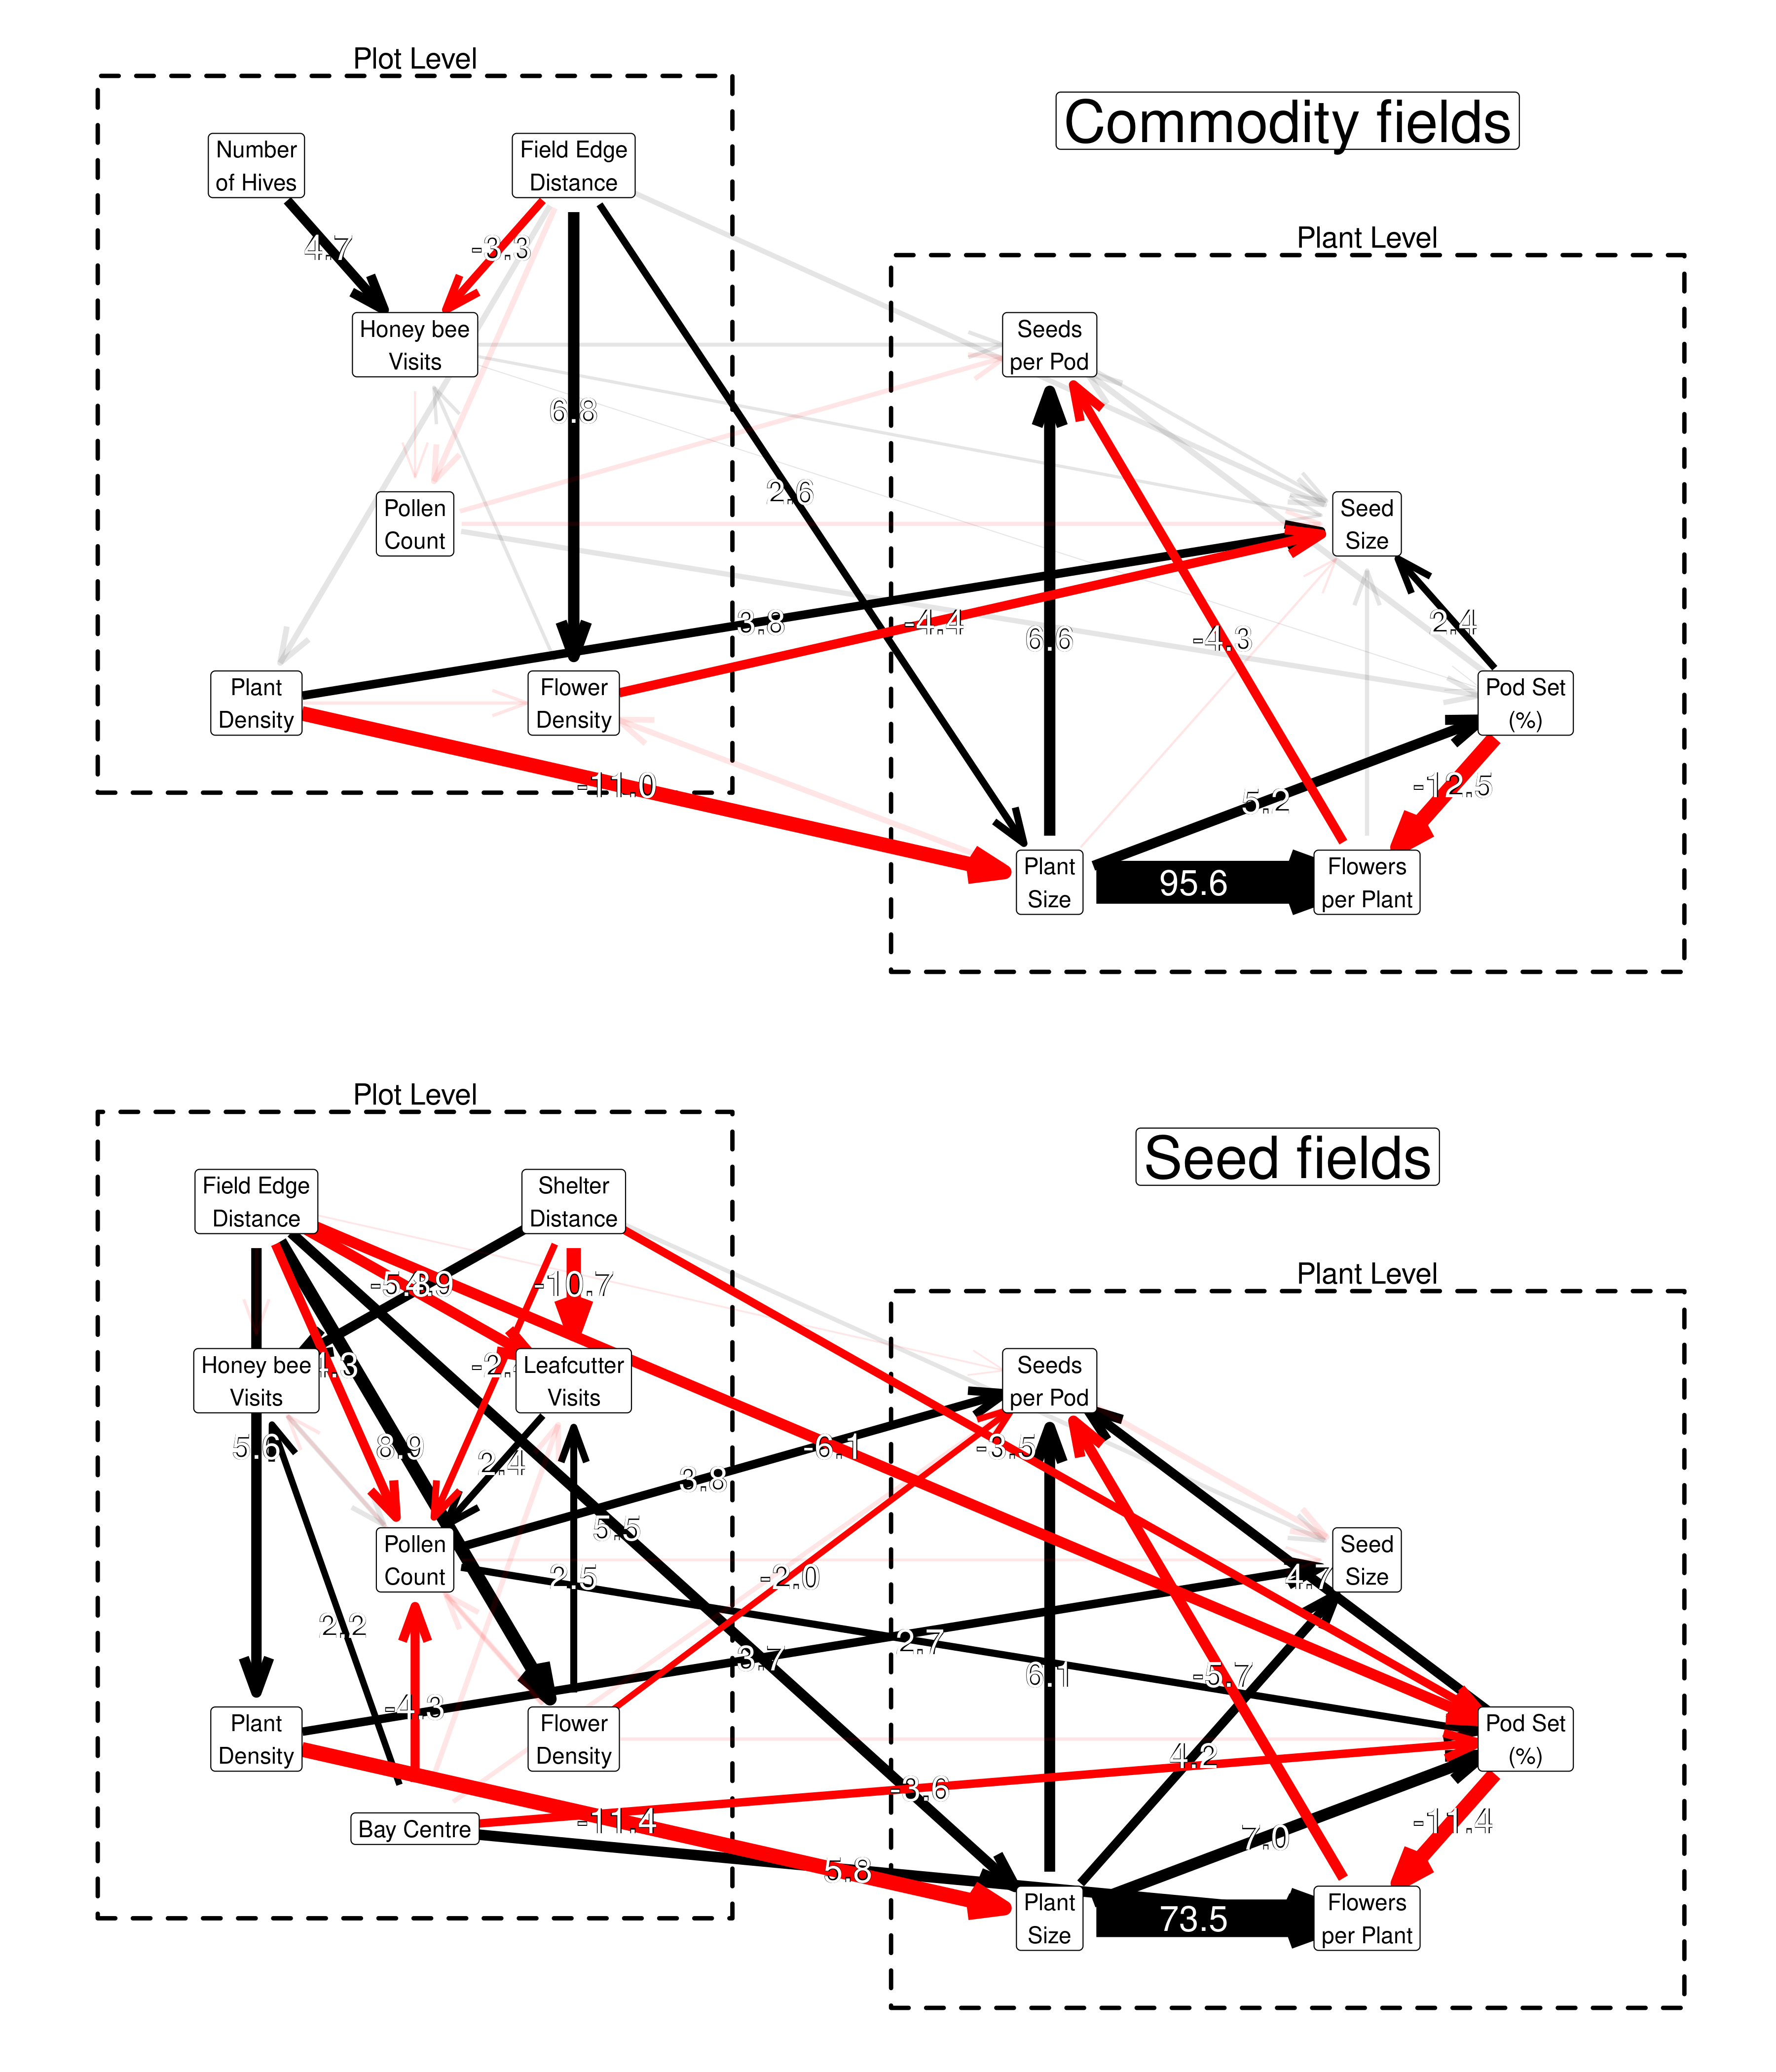
\includegraphics[width=\textwidth,keepaspectratio=true]{../Figures/allSEM.png}
    \caption{Results of path analysis in commodity and seed fields. The width of each arrow is proportional to the effect size of each component path (number also displayed). Transparent arrows show path coefficients whose 95\% posterior intervals overlapped zero.}
    \label{fig:allSEM}
\end{figure}


\subsection*{Visitation}

Honey bee visitation decreased with distance away from the edge of the field in both commodity and seed canola fields.
In commodity fields, HB visitation decreased from 12 visits/hr at the edge to 1.8 visits/hr at 400 m into the field (Figure \ref{fig:allVisits}a, apiary of 40 hives).
Lower stocking rates decreased HB visitation at the edge of the field to 7.4 visits/hr at 20 hives, while unstocked field edges had an average of 0.8 visits/hr.
Unsurprisingly (given the higher stocking rate of 160 hives per field), HB visitation was much higher in seed canola fields, and decreased from 96.4 visits/hr at edge to 85.7 visits/hr at the centre of the field (Figure \ref{fig:allVisits}a). 
Visitation was also much lower near LCB shelters, dropping from 81 visits/hr at 20 m to 31 at 2 m (Figure \ref{fig:allVisits}b), likely due to competition with LCBs.
% Visitation rates were higher in both years in Lethbridge (2014: 9.3 visits/hr, 2015: 7.1), but were higher in 2015 than 2014 at Grande Prairie (Z=2.3, p$=$0.02), rising from 5 visits/hr at the field edge in 2014 to 17 visits/hr in 2015. % (at a stocking level of 20 hives). 

LCB visitation was much higher close to their shelters, and surprisingly, was also higher at the edge of the field.
LCB Visitation dropped from 350 visits/hr at 2 m from the shelter to 50 visits/hr at 20 m (Figure \ref{fig:allVisits}b), and also decreased from 119 visits/hr at the edge of the field to 25 at the centre (Figure \ref{fig:allVisits}a, b)
The difference in LCB visitation between the edge and centre of the female bays was weak (p=0.14), while HB visitation was higher at the centre of the bay (88 vs. 139 visits/hr, Figure \ref{fig:allVisits}b), indicating that pollination is likely done by different species in different parts of the field.
% There was no difference in visitation rates between the male bay and the edge of the female bays (LCB: p$=$0.72, HB: p$=$0.32). 
% However, there was no difference in visitation rates between the edge and the centre when LCB cocoon stocking was lower (Z=2.2, p$=$0.028), indicating that LCBs at high stocking densities likely aggregate in shelters close to the edge of the field (Figure \ref{fig:hbeeDist_both}).
%Therefore, visitation by both species strongly decreases with distance from the edge of the field, decreases with distance from the leafcutter shelters in seed canola fields, and is done by different bees at the centre of the female bay.

\begin{figure}
    \centering
    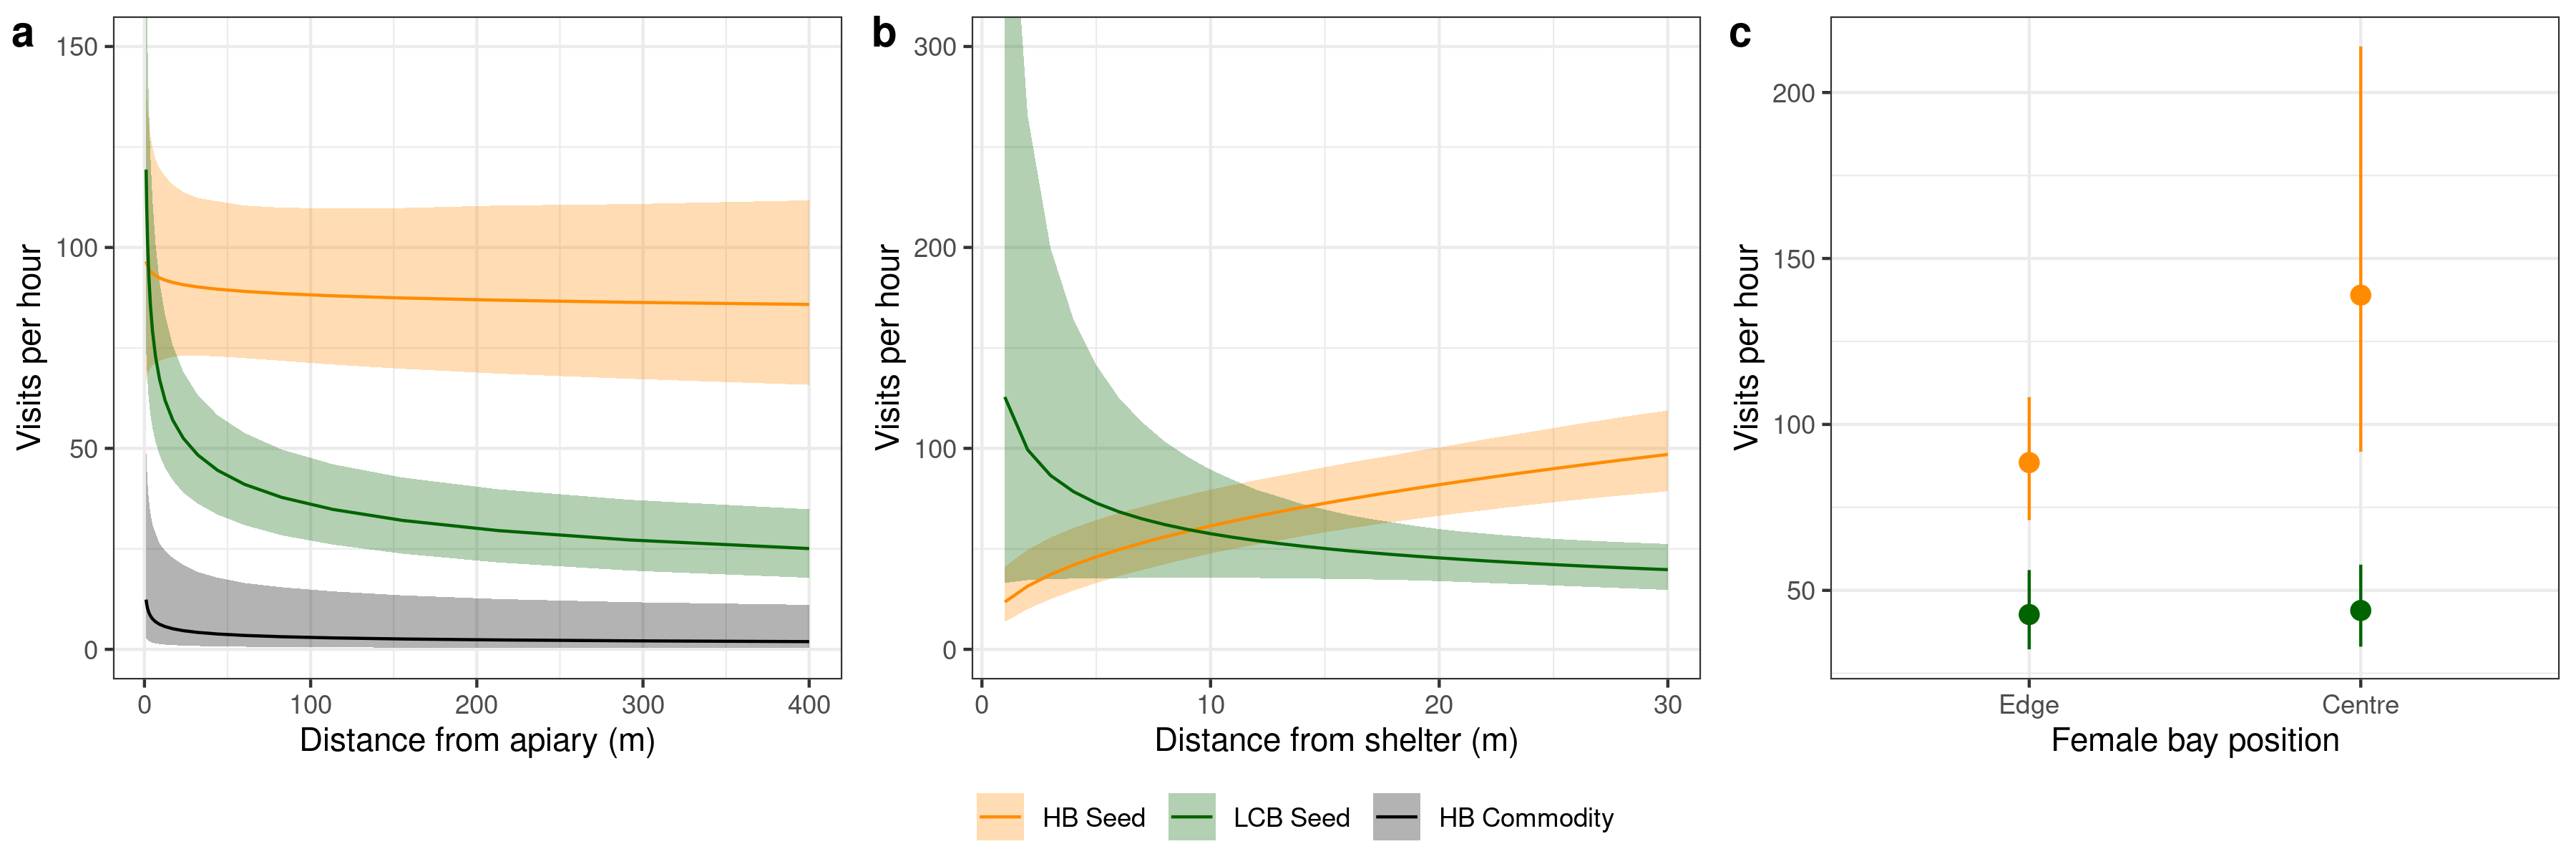
\includegraphics[width=\textwidth,keepaspectratio=true]{../Figures/allVisits.png}
    \caption{Effect of distance from a) honey bee apiaries, b) leafcutter shelters, and c) female bay position on visitation rates. Commodity fields are shown at a stocking rate of 40 hives (black line), while stocking rates are at 160 hives in seed fields (yellow line).}
    \label{fig:allVisits}
\end{figure}

\subsection*{Pollen Deposition}

LCB visitation increased pollen deposition in seed canola fields, but honey bees did not increase pollen deposition in commodity or seed canola fields.
Pollen deposition on stigmas was high in commodity canola (mean: 293 grains/stigma, SD: 385, range: 0--3981), but honey bee visitation had no impact on this (p$=$0.77, Figure \ref{fig:allPollen}a).
Pollen deposition declined weakly with distance from the edge of the field (p$=$0.09), but this only amounted to a 6\% average decrease (290 grains/stigma at the field edge vs. 240 at field centre).
In seed canola, pollen deposition was much lower overall (mean: 22 grains per stigma, SD: 43, range: 0--578), and decreased from 26.3 grains/stigma at the edge to 11.5 at the centre of the field (Figure \ref{fig:allPollen}b) independent of visitation.
LCB visitation increased pollen deposition from 13 grains/stigma at 0 visits/hr to 25 pollen grains at 100 visits/hr (Figure \ref{fig:allPollen}a), but there was no effect of honey bee visitation (p$=$0.20), implying that most of the pollen deposition in seed fields is the result of LCB visitation.
Pollen deposition also decreased from 15 grains/stigma at the edge of the female bay to 9 at the centre of the bay independent of visitation, suggesting that pollen may be lost from bees crossing over from male bays.% \citep{pinnisch1990}.%, who likely visit flowers at the edge of the bay first. 
% Flies were also common visitors in commodity fields (Table \ref{tab:propVisitors}), but had no effect on pollen deposition (p$=$0.577), so only honey bees and LCBs were considered as potential pollinators (other flower visitors were rare).

\begin{figure}
    \centering
    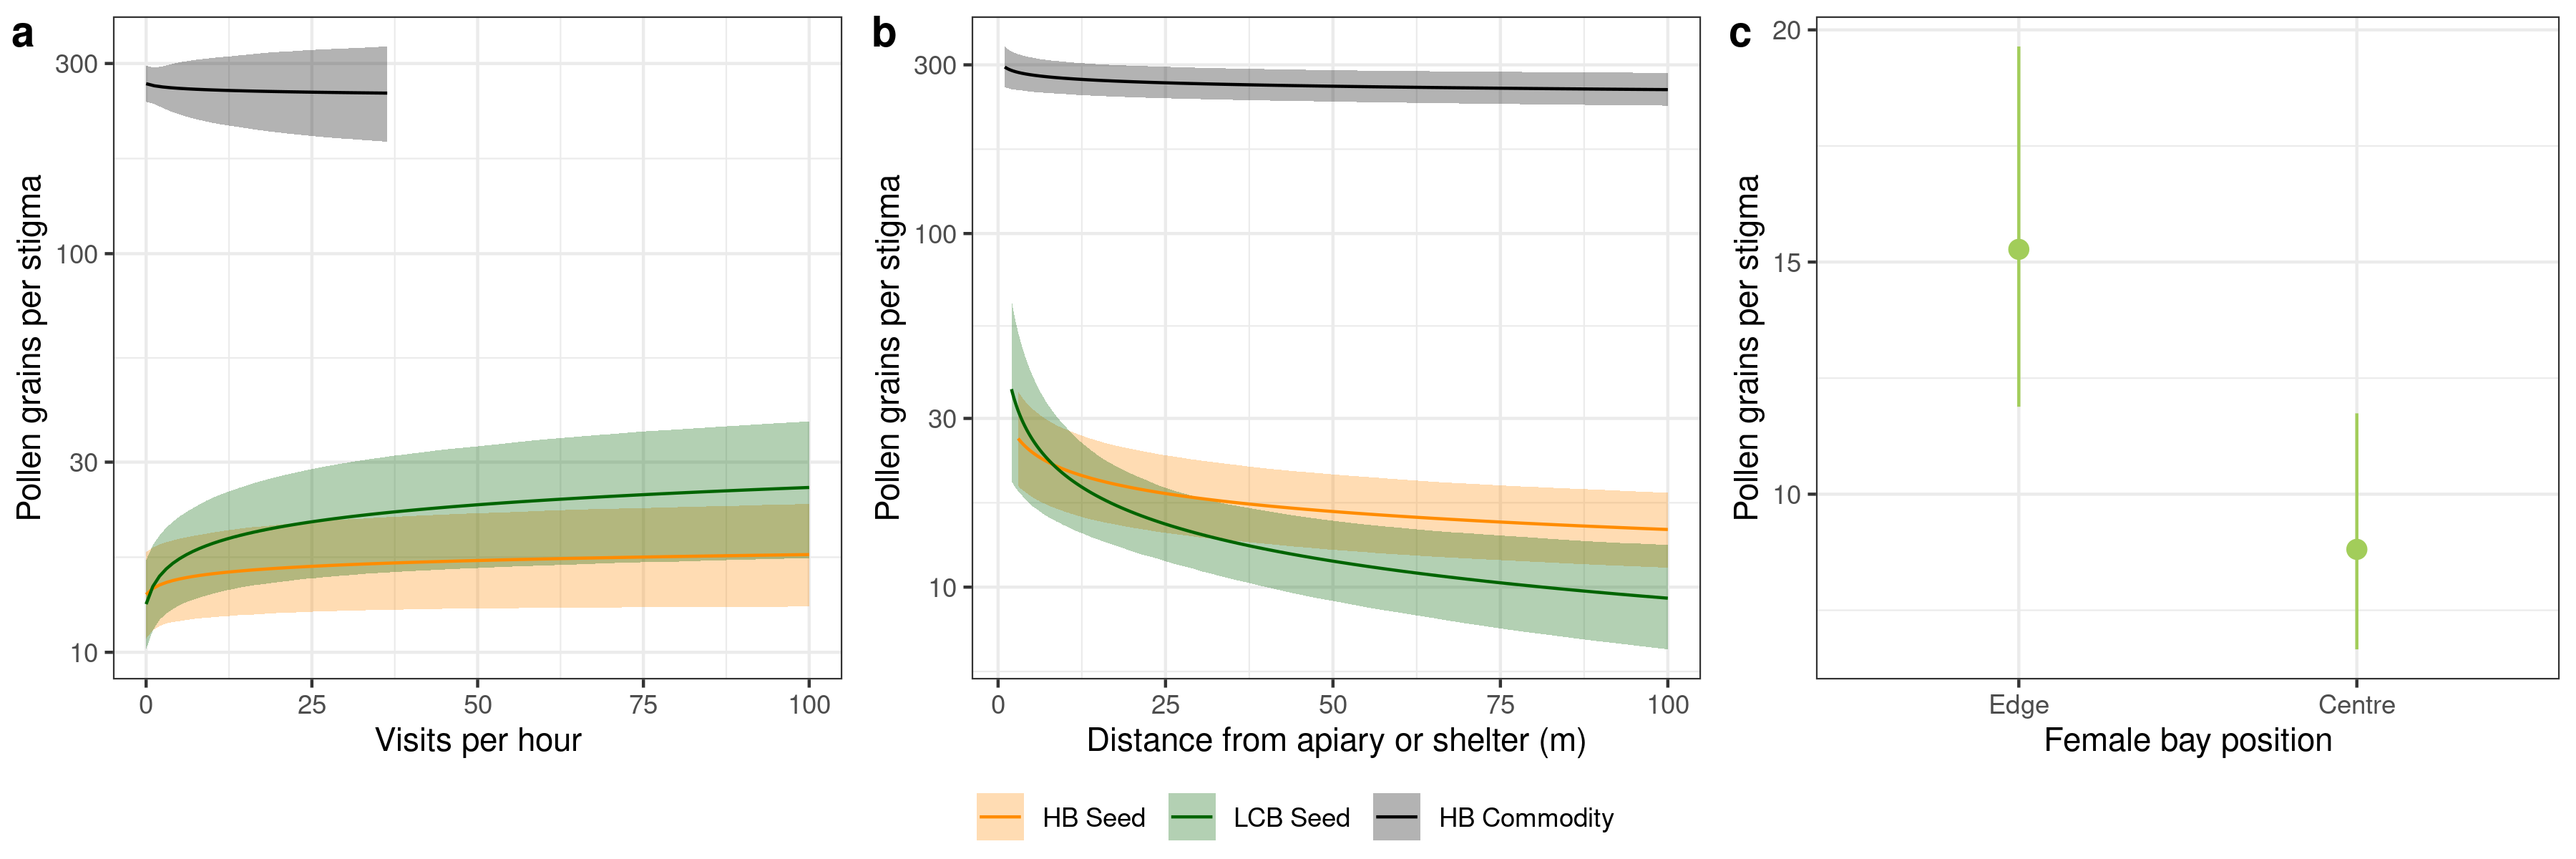
\includegraphics[width=\textwidth,keepaspectratio=true]{../Figures/allPollen.png}
    \caption{Effect of a) visitation rate, b) distance from apiary (HB) or shelter (LCB), and c) female bay position on pollen deposition.}
    \label{fig:allPollen}
\end{figure}


\subsection*{Seed Production}

% % Not sure that this paragraph needs to be here - move to Appendix
% Plant size was influenced by plant density, but this differed between commodity and seed canola crops.
% Plant density was higher overall in commodity fields (mean: 48.5 plants/m$^2$, SD: 22.9, range: 6--151 ) than seed fields (mean: 39.4 plants/m$^2$, SD: 17.0, range: 11--89), and commodity canola plants were smaller on average (mean: 18.2 g, SD: 14.4, range: 0.8--110.2) than seed canola plants (mean: 30.7 g, SD: 21.2, range: 1.2--144.3).
% Plant size was negatively influenced by plant density in seed canola fields (Z=-13.2, p$<$0.0001), but not in commodity canola fields (Z=-1.62, p$=$0.10, Figure \ref{fig:plDensPlSize}), indicating that density-dependence is more variable in commodity fields. 
% Plants were larger at the centre of the field independent of density (Z=5.4, p$<$0.0001).%, possibly because of proximity to the centre of the irrigation system. 
% Plant density was slightly lower at the edge of commodity canola fields (Z=1.68, p=0.09), but was much lower in seed canola (Z=5.2, p$<$0.0001), indicating lower seedling survival at the edges of the field.
% Neither irrigation (p=0.76), site (p=0.86), nor distance from field edge (p=0.70) directly influenced commodity canola plant size, but plants were larger in 2015 (Z=2.5, p=0.01). 

\begin{figure}
    \centering
    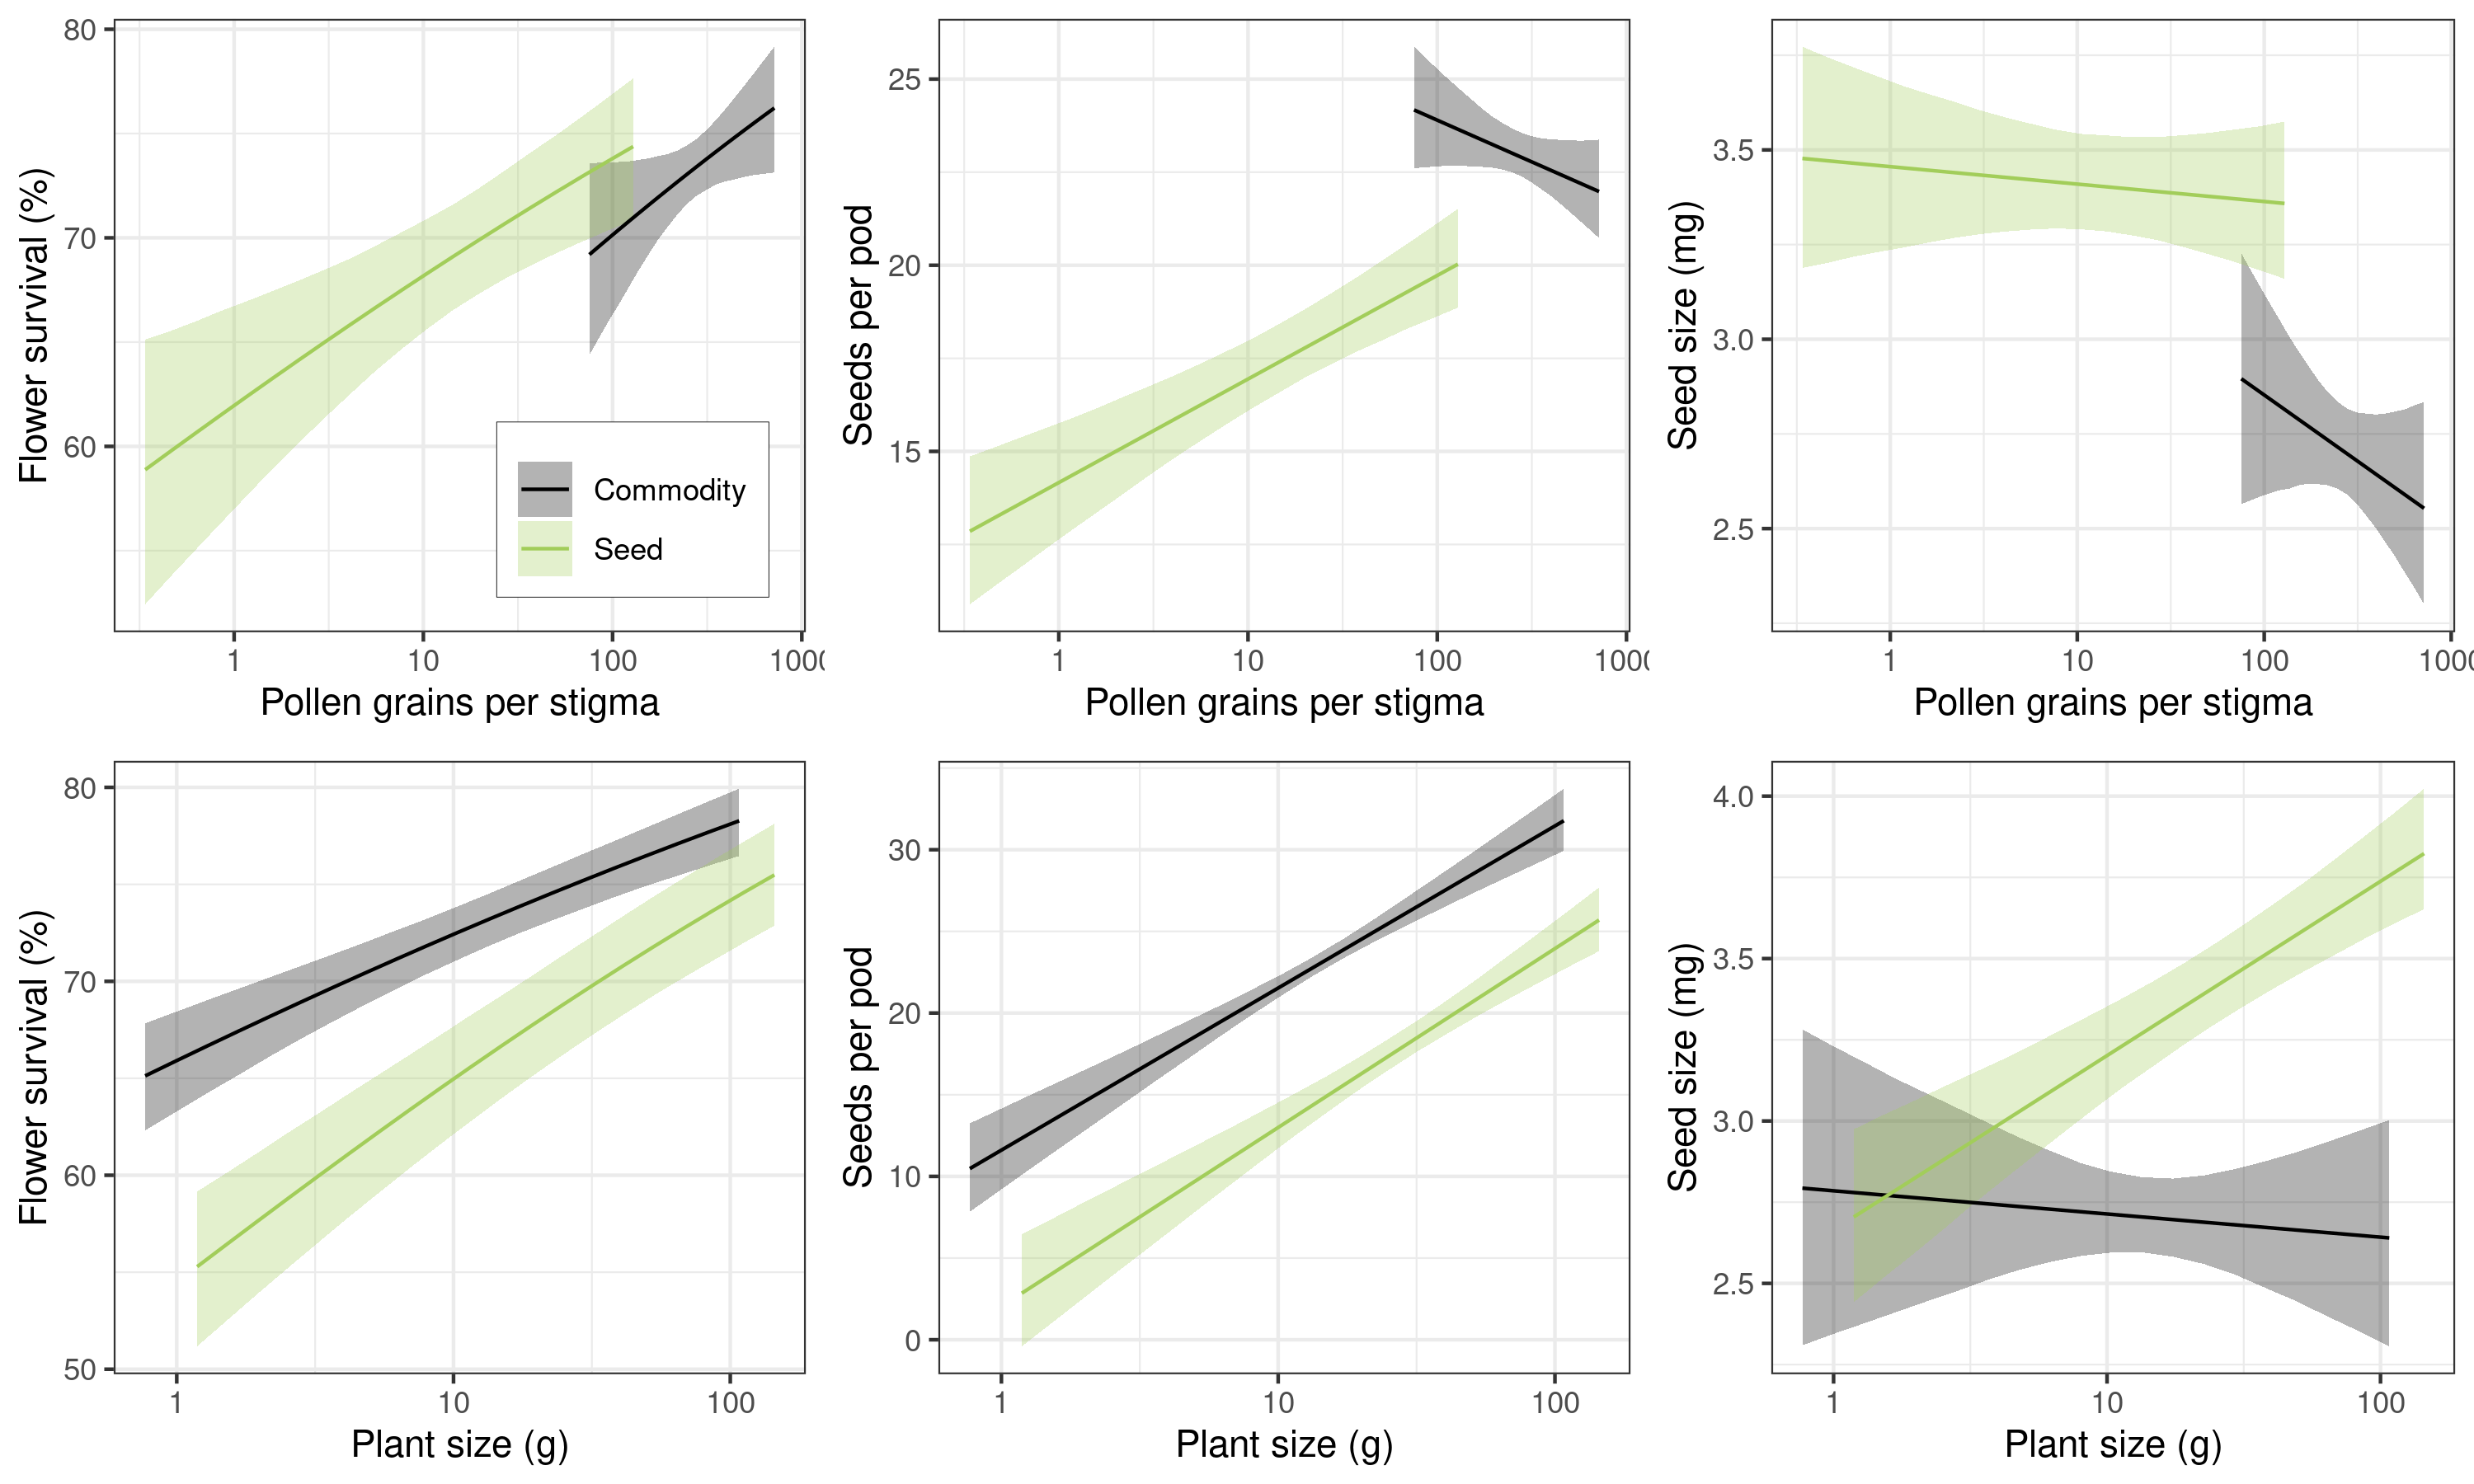
\includegraphics[width=\textwidth,keepaspectratio=true]{../Figures/allSeeds.png}
    \caption{Effect of pollen deposition (top row) and plant size (bottom row) on flower survival, seeds per pod, and seed size.}
    \label{fig:allSeeds}
\end{figure}

Commodity canola produced fewer flowers per plant than seed canola (mean: 196 vs. 461), and also produced fewer pods per plant (143 vs. 299, Table \ref{tab:dataSummary}).
Commodity canola also produced more seeds per pod than seed plants (mean: 23 vs 16), but seed size was lower in commodity canola (2.74 vs 3.43 mg/seed). 
Finally, commodity plants were also lower-yielding than seed canola plants (mean: 6.8 vs 9.5 g seed per plant), but produced more seeds per gram of vegetative biomass than seed canola plants (mean: 0.38 vs. 0.32), likely due to lower pollen limitation.

Plant size had by far the strongest positive effect on the number of pods produced, and there was evidence of pod set suppressing flower production (see plant paths in Figure \ref{fig:allSEM}), but pollen only directly affected production in seed canola.
In both commodity and seed canola, plant size had a strong positive effect on the total number of flowers per plant as well as \% pod set (Figure \ref{fig:allSeeds} bottom row), but did not increase seed size in commodity canola.
Plant density also had a positive direct effect on seed size in both crops, indicating that areas with better resources can support better-provisioned (but smaller) plants.
Pod set also had a strong negative influence on flowers per plant in both crop types, indicating that high pod set suppresses future flower production.

Pollen deposition did not alter seed production in commodity canola, nor was there a direct effect of honey bee visitation or distance from field edge (note log-scaled x-axis on Figure \ref{fig:allSeeds}).
Pod set and seeds per pod in seed canola were increased by higher pollen deposition, and decreased with distance away from HB hives as well as distance from LCB shelters.
Pod set was also lower in the centre of the female bay, again suggesting that pollen is lost when bees crossing over from male bays.

\subsection*{Yield simulations}

The path analysis simulations further confirmed the results of the analysis: HB visitation had little effect on yield in either crop type, but LCB visitation improved yield in seed crops.
The simulations showed no large effect of HB stocking on seed size or total yield in commodity fields (Figure \ref{fig:allYield}a, b), aside from the effect associated with distance from the edge of the field.
Similarly, the simulations for seed fields showed a small increase in seed size and total yield with distance from the HB hives at the field edges, but the effect of distance from the leafcutter shelters was much more dramatic (compare the spacing of isolines along the x-axis and y-axis in Figures \ref{fig:allYield}c, d).
A second set of simulations were run only in seed fields, in order to compare the effect of pollinator distances between the bay edge and centre. 
This revealed that not only total seed size and overall yield lower at the bay centre, but that the effect of HB distance is effectively \emph{nil} at the bay centre (yield isolines are essentially horizontal in bay centre, and slightly tilted at the bay edge, Figure \ref{fig:allYield}d, f).
Interestingly, the simulations also showed evidence of nonlinear behaviour occurring in the centre of seed field bays, where a local minima in yield appears at approximately 25 m away from HB hives and 45 m away from LCB shelters (Figure \ref{fig:allYield})f), likely because of an interaction between the components of yield (seeds per pod, pods per plant, and weight per seed). 

\begin{figure}
    \centering
    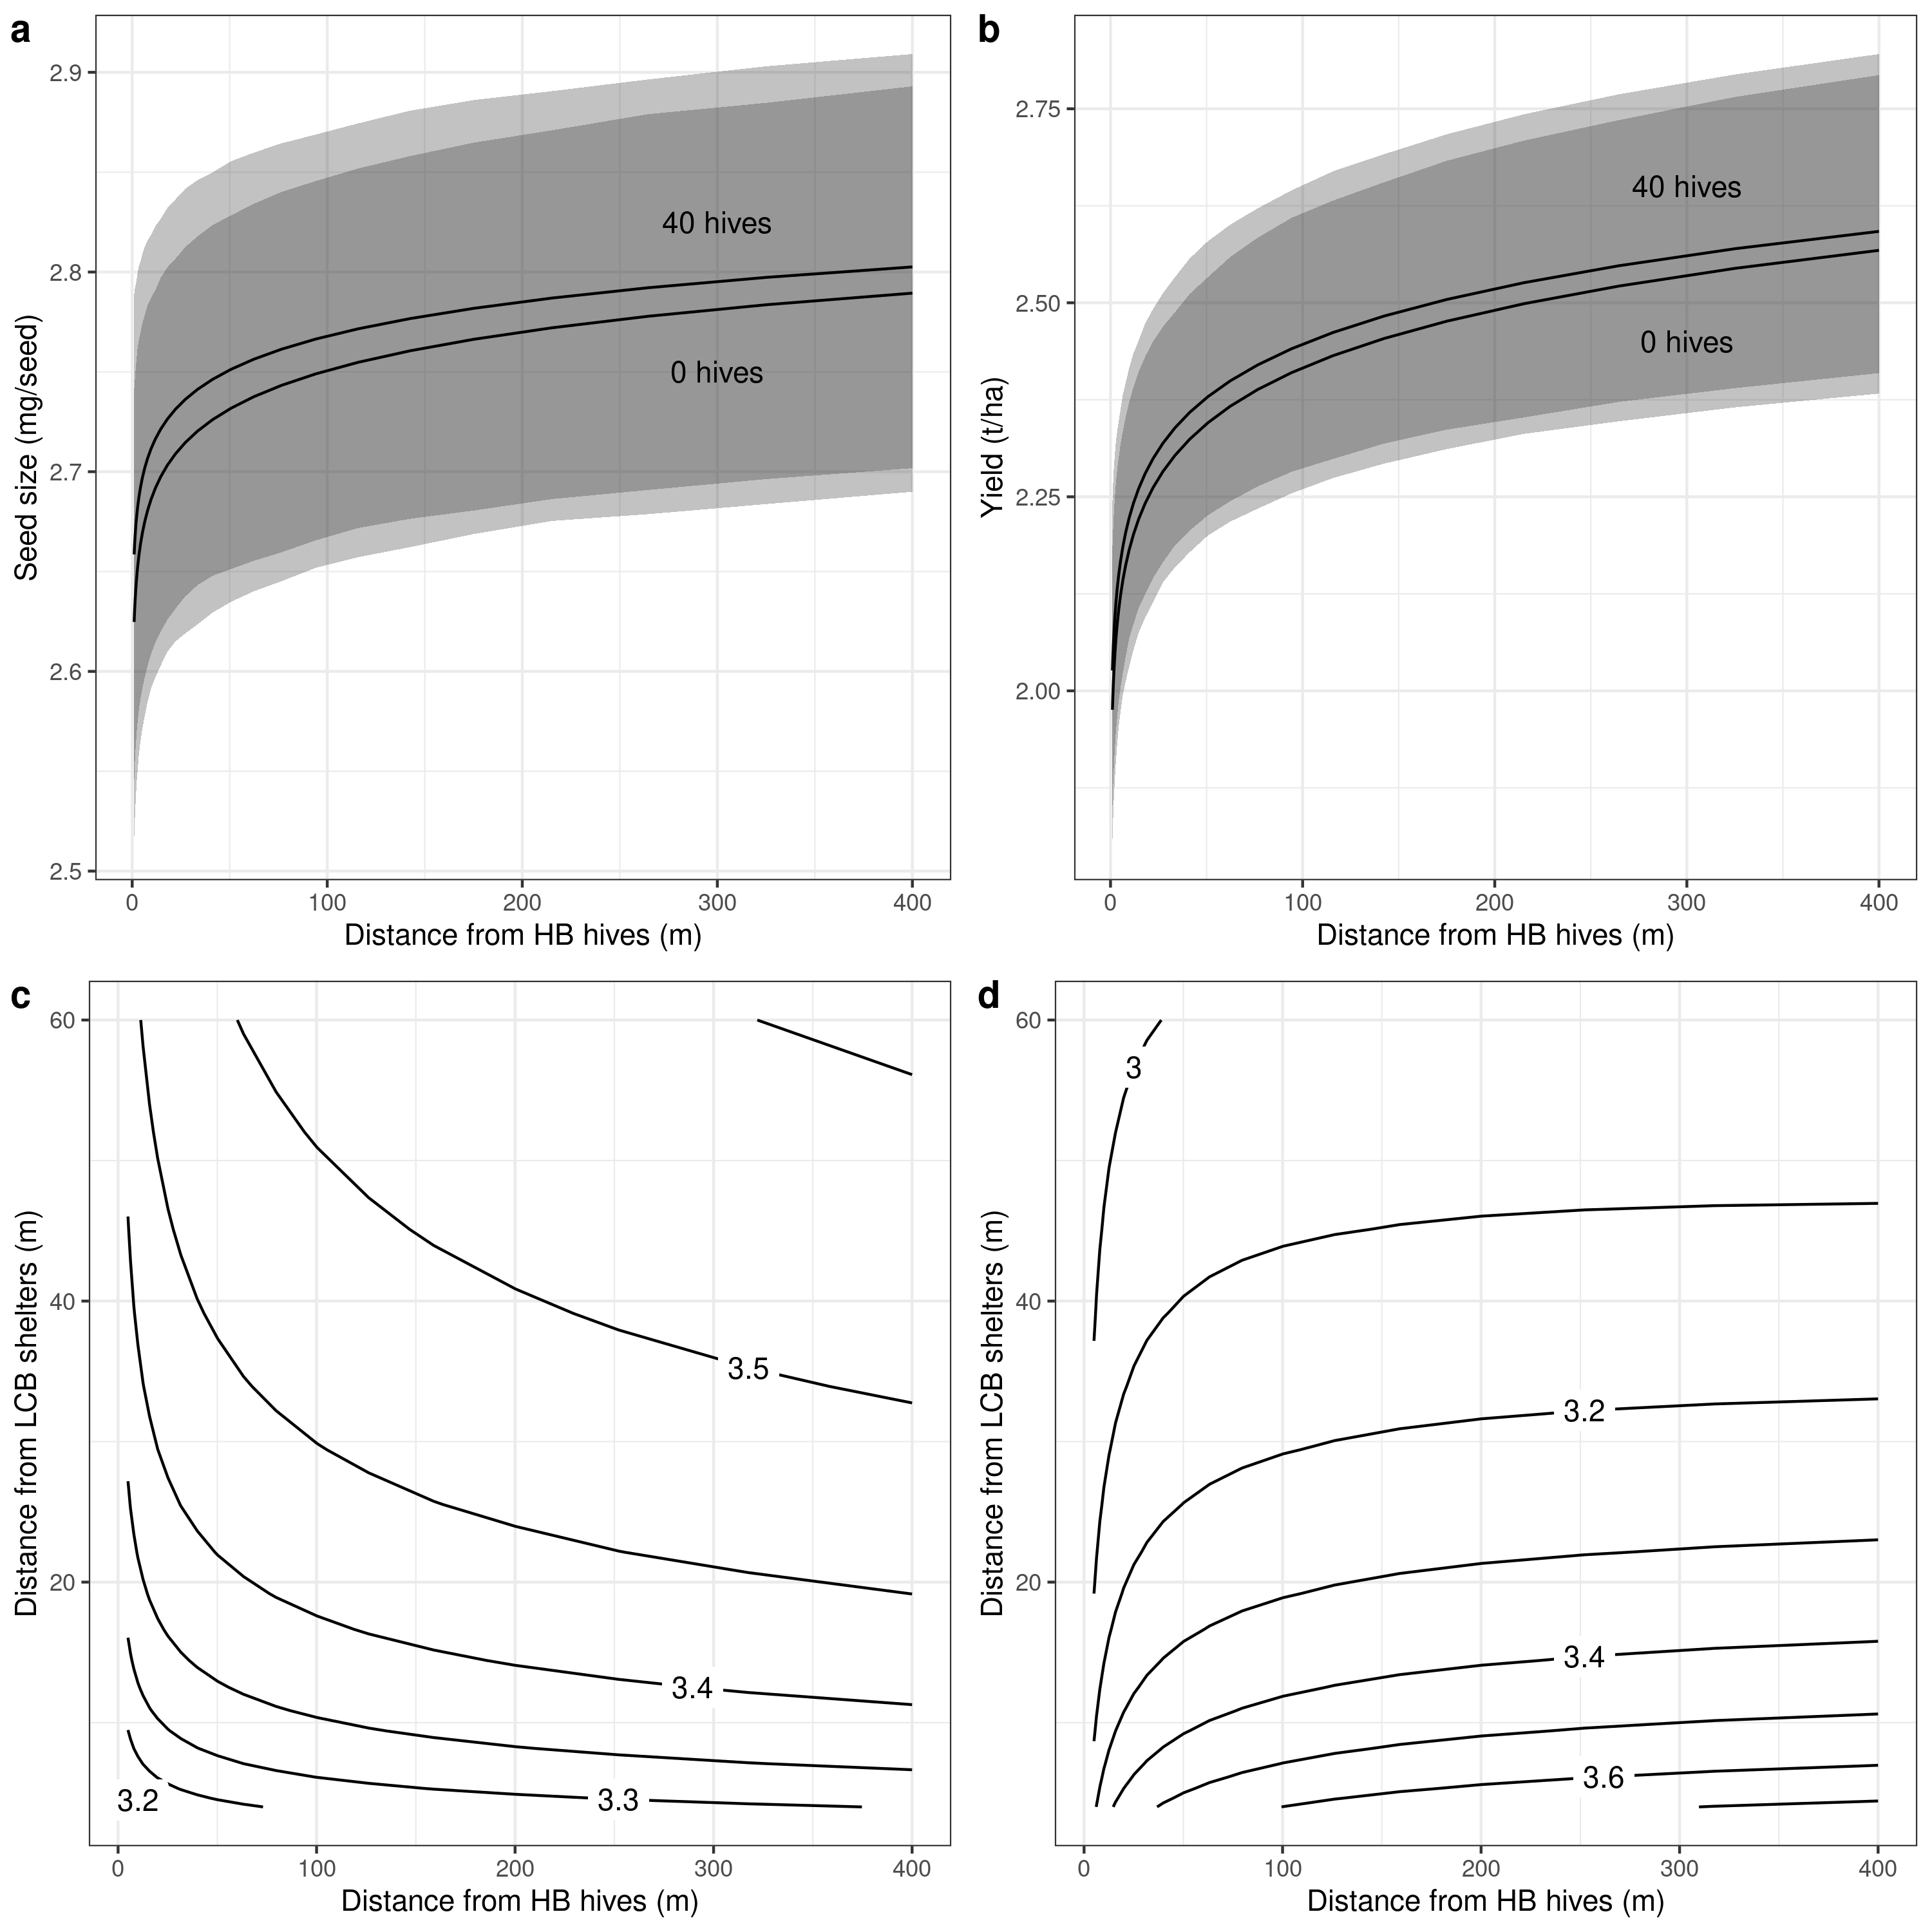
\includegraphics[width=\textwidth,keepaspectratio=true]{../Figures/allYield.png}
    \caption{Effect of honey bee distance and leafcutter distance on seed size (first column) and total yield (second column), using coefficients from paths for simulation, while holding plant density constant at its mean value. Shaded areas shown in a \& b are 95\% quantiles for the simulations. Lines on panels c - f are isolines of constant seed size (c, e) or yield (d, f).}
    \label{fig:allYield}
\end{figure}

\section*{Discussion}

We examined how bee visitation contributes to pollen deposition and seed yield in two canola crops, and showed a strong link between visitation and yield in seed canola, but not in commodity canola.
HB and LCB visitation decreased with distance from their respective hive or shelter, but unexpectedly, LCBs were found more at the edge of the crop.
HB visitation had little direct influence on pollen deposition in either crop type, while LCB visitation had a positive effect on pollen deposition in seed canola.
We found that commodity canola production is largely limited by plant size, while seed canola production is limited by both pollen and plant size.
Finally, our simulation results from the path analyses confirmed this, and showed the strong influence of LCB visitation on seed size and yield.
These results provide more realistic information on the value of pollination services in commodity and seed canola crops, and show how a statistical-mechanistic model of seed production provides richer insite into the process of seed production than linear models alone.

\subsection*{Bee visitation} 

HB visitation in both field types declined with distance into the field, but overall visitation was much higher than commodity fields, due to the higher HB stocking rate used in seed fields (3.6 vs. 0.6 hives/ha).
Since HBs travel from their hive outside the edge of the field, this decline was not surprising, but we did not expect a similar decrease in LCB visitation with distance into the field, as their shelters are located \textit{within} the field.
This decrease with distance into the field may have been caused by LCBs migrating from shelters at the centre of the field to the edge \citep{goerzen1995}, as female LCBs are central-place foragers, and tend to not forage far from their nests \citep{peterson2005,pitts2011, brunet2019}.
However, LCBs are not as constrained to a single nest as HBs are, and can drift between shelters within a given field \citep{goerzen1995, pittsSinger2013}.
LCBs must also forage for leaf materials to create cocoons, but prefer thinner, non-canola leaf types, mainly plants in the families Fabaceae and Rosaceae \citep{sinu2018}.
Since seed canola fields have very few weeds within the area of the crop, LCBs at the centre of the field may have few choices of leaf material, or alternative pollen and nectar sources.
Therefore, LCBs likely move from the shelters at which they were released to the shelters at the edge of the field, so as to gain access to better leaf material or different sources of pollen and nectar \citep{horne1995, horne1995b}.
% To test this, a mark-recapture study of female LCBs could be done to see if bees migrate to shelters at the edge of the field, or if visitation is higher due to other reasons (\textit{e.g.} feral populations migrating to edge of field, long-distance foraging from centre of field as in \citealp{peterson2005}).  %SH: FINE FOR THESIS, BUT CAN BE REMOVED FOR MANUSCRIPT
% This would explain why LCB visitation was higher at the edge of the field, and may also explain why this pattern was not seen in fields with half-stocked shelters.
% It would be interesting to see if there is a critical threshold of LCB density per-shelter that causes them to move to shelters at the edge of the field (similar to \citealp{pittsSinger2013}).
%HBs visited flowers at the edge of the field more frequently than those in the middle of the field, as predicted for central-place foragers with nesting aggregations outside the field (\citealp{olsson2014}, see Chapter 2).
%Similarly, the high concentration of canola nectar (\citealp{mohr1990}, 58.3\% brix from Chapter 2) may cause leafcutter bees to choose more diluted nectar under hot and dry conditions, similar to HBs \citep{ohguchi1983}. % canola pollen is valuable to bees \citep{mohr1988,huang2004},
% Potential future studies should investigate how leafcutter bees shift among shelters after emergence, how cocoon production in seed fields varies with distance, and should investigate inter-cropping leaf material plants (e.g. \emph{Polygonum}, \emph{Pisum}, or other large, thin-leaved plants) to encourage leafcutter bees to stay within the field.

%Leafcutter-honeybee interactions
In seed fields, LCB visitation was higher, and HB visitation was correspondingly lower in areas close to LCB shelters. 
Lower HB visitation may have been driven by lower nectar and pollen resources, as areas close to leafcutter shelters can become depleted in nectar and pollen \citep{currie1997}.
HBs also suffer from direct interference by LCBs near to their shelters; during the study we observed LCBs directly harassing HBs during the plot-level observations, attacking HBs both on the flowers and in the air (also seen by \citealp{batra1978} and \citealp{waytesMsc}). 
HB visitation and foraging behaviour varied strongly between the edge and centre of the female bays in seed fields, while there was little difference between LCB visitation rates.
HB visitation rates were almost twice as high at the centre of the female bay, likely reflecting a stronger need for pollen among LCBs than HBs \citep{cane2011} (although interestingly, there was also no difference in LCB visitation between male and female bays).

Very few HBs in the female bay were pollen foragers (1.4\%, see Table \ref{tab:sideWorking}), meaning that foragers who have (recently) come into contact with pollen rare.
Both \citet{waytesMsc} and \citet{gaffney2019} showed that HBs exhibit floral fidelity during foraging trips, with minimal crossing between male and female bays ($\sim$5\% of observations, \citealp{waytesMsc}), limiting pollen transfer between the male and female flowers.
Side-working was a very common behaviour among HBs in commodity fields (65\% of the total visits from HBs during 2015 were side-working), as well as the male bays of seed fields (36\%), but not in the female bays (3\%, Table \ref{tab:sideWorking}).
This behaviour is relatively common on male-fertile flowers of \textit{Brassica} \citep{free1973,free1983,delbrassine1988,mohr1988} as well as other flowering crop flowers \citep{thomson2001}, and may be due to HBs avoiding contact with the stigmas to increase ease of access to nectar, or to reduce the amount of grooming needed during a nectar foraging bout.
The foragers who were side-working tended to not switch to top-working (personal observation), so this is likely a consistent individual behaviour (at least in experienced foragers).
Taken together, these pieces of evidence suggests that HBs have limited opportunities for pollen transfer in both commodity and seed fields, as they commonly engage in side-working behaviour in both field types, and pollen foragers typically avoid female bays in seed canola fields.

%However, after controlling for stocking rates, visitation in commodity fields was higher in Grande Prairie in 2015.
%This may have been caused by greater food availability outside of canola fields in 2015, causing foragers to concentrate in canola fields.
%Canola nectar tends to have high sugar concentrations \citep{szabo1985}, so workers may have selected lower-concentration flowers in field margins and ditches, such as \textit{Trifolium} and \textit{Medicago}, instead of the flowers in the canola fields, depending on local abundances in each year and location, but this seems unlikely, as nectar concentrations were higher in 2015 in Grande Prairie (Chapter 2 Appendix).
%Water foraging differences between years may also help to explain this effect, as foraging HBs tend to avoid concentrated nectar or prioritize water foraging \citep{lindauer1955,kuhnholz1997} during hot weather.
%During 2015, we did notice a large number of foragers in Lethbridge gathering water from pools of water near fields instead of visiting flowers (personal observation), so foragers may have been gathering water instead of foraging on flowers (at least in that region), but this is anecdotal, and would require a formal study to confirm this. 
% Avoidance of concentrated nectar may reflect slower rates of imbibing them \citep{harder1986}.
% Nectar concentrations were slightly higher in GP in 2015 (60 vs 56), but were about 58.4 each year in LB. Soil water and irrigation don't appear to do much (ultimately needs better modelling, though)

\subsection*{Pollen deposition}
%Pollen deposition in commodity fields
HB visitation did not increase pollen deposition in commodity canola fields compared to unstocked fields, meaning that wind and/or self-pollination are the likely agents of pollen transfer.
The stigmas and flowers of \emph{Brassica} are not aligned for dispersal and deposition from the wind, so cross-pollination likely occurs mainly via insects \citep{mesquida1982,cresswell2004}.
However, wind-induced self-pollination (plant shaking) can increase yield in \textit{Brassica} \citep{williams1986, mesquida1988c}, and fields without bee pollination have outcrossing rates of about 20\% within the field \citep{rakow1987,becker1992}.
% The style of \textit{Brassica} grows past the anthers during maturation, allowing deposition of large amounts of self-pollen, suggesting that self-pollination is the dominant mode of pollination.
HBs can assist in deposition of self-pollen, as \citet{ali2011} found that \textit{Apis dorsata} and \textit{Apis florea} can both deposit 100-200 grains of pollen per visit on a canola flower (\emph{B. napus} var. \emph{Bulbul}).
However, \citet{waytesMsc} used male-sterile flowers from seed canola fields and found that HB pollen foragers deposited far less outcrossed pollen ($\sim$ 2 grains per visit), suggesting that much of the pollen deposited on commodity canola stigmas may be self-pollen. 
Because the overall pollen deposition rates found in this study were high, HB visitation seems to have made little difference in the amount of self-pollination, as large amounts of pollen were present on commodity canola stigmas even at the centre of unstocked fields.
This suggests that commodity canola stigmas are largely saturated with self-pollen, swamping any extra pollen deposition by HBs.
% The typical lifetime of a canola flower is approximately 3 days, and the stigmatic surface is receptive for 24--36 hours within this period \citep{eisikowitch1981,hoyle2007}, so it may be that 10-minutes of observing flower visitors was too short of a time interval to relate to pollen deposition.
% This is unlikely, however, 
%SH: DOING A BACK-OF-ENVELOPE CALC: 0.23 VISITS/HR X 2 GRAINS/VISIT X 12 HR X 3 DAYS = 5-6 GRAINS PER DAY, LESS THAN 1% OF STIGMA LOAD
% This runs contrary to other studies in commodity canola (\citealp{sabbahi2005}, but see \citealp{garibaldi2013} and \citealp{waytesMsc}), so why did 

Our models also showed that pollen-transferring behaviour of HBs is limited in seed fields, as deposition strongly increased with LCB visitation but not HB visitation.
HBs in seed fields tended to visit more in the centre of the female bay, even close to the edge of the field, yet pollen deposition was still about 40\% lower.
LCBs switch between male and female flowers more frequently than HBs, travel further between flowers, transport more viable pollen, and tend not to side-work canola flowers \citep{soroka2001, parker2015, waytesMsc, brunet2019}, all of which may explain their higher pollination efficacy.
Pollen deposition in seed fields also decreased with distance from the edge of the field, and was lower in the centre of the female bays independent of visitation, suggesting lower pollen tranfer per visit.
These may have been caused by two separate processes: a) low pollen carryover with distance into the female bays, and b) shorter trips between flowers at the centre of the field.
Pollen carryover from the edge to the centre of the bay female is likely reduced as LCBs typically visit the edge of the female bay before venturing into the centre \citep{thomson1986, pinnisch1990}.
\textit{Bombus} take shorter trips between flowers under nectar-rich conditions \citep{pyke1978b, heinrich1979}, suggesting that HBs and LCBs may operate similarly at the centre of seed fields, resulting in lower pollen transfer.
While manipulating nectar levels within a field to produce greater travel between flowers could be extremely difficult, this suggests that the optimal width of female bays within seed fields may be lower than is currently practiced.

While we found that HBs have no direct effect on pollen deposition in either crop type, they may have an indirect positive effect caused by: a) increasing airborne pollen from male-fertile flowers \citet{pierre2010}, b) lowering nectar and pollen standing crop, causing LCBs to travel further \citep{pyke1978b, heinrich1979}, or c) lowering floral fidelity on higher-rewarding flowers in the male bays \citep{mesquida1978, waytesMsc,gaffney2019}.
A simple test of this might be to remove HB hives from a seed field (mid-season) and observe changes in LCB visitation before and after the removal.

\subsection*{Seed production} % The total yield of a canola plant is a function of three components: number of pods per plant, number of seeds per pod, and seed size.

% Plant size was the only important factor in commodity canola seed production (i.e. pod set, seed size, and seeds per pod), but both plant size and pollen deposition were the main drivers of production in seed canola.

Plant size increased the rate of pod set in commodity canola, but both plant size and pollen increased pod set in seed canola, suggesting that both pollen deposition and plant resources constrain pod production.
This is similar to the findings of \citet{mesquida1981} and \citet{steffan2003}, who found that pod set in male-sterile plants responded positively to visitation, while male-fertile plants had no response (but see \citealp{adegas1992}).
Both pod set and seeds per pod can increase with extra pollination \citep{jauker2008,sabbahi2005,sabbahi2006,duran2010}, so the low influence of pollination in commodity fields may be due to a high overall level of pollen deposition (Figure \ref{fig:allPollen}).
There was no additional effect of HB visitation on pod set, meaning that that HB visitation did not cause more pollen deposition or improve its quality through increased outcrossing (as in \citealt{rosa2011}), but this may depend on the variety \citep{adamidis2019}.
Flowers per plant was reduced by pod set, implying that high pod set suppresses further flower production or increases competition among pods for plant resources.
The first scenario is more likely, as \citet{sabbahi2006} and \citet{mesquida1981} both found that canola plants compensated for experimental removal of flowers by increasing branch and flower production, until the plant reached about 170 pods.
There were also effects of distance on pod set independent of pollen: pod set decreased with distance from the edge of the field, distance to LCB shelters, and was lower at the centre of the female bays.
\citet{mesquida1978} also found that pod set in male-sterile canola declined quickly with distance from the male-fertile plants (due to wind pollination), but the effect we found is likely related to the earlier effect of lower pollen carryover at the centre of the female bays, and possibly the centre of the field.
Finally, the effect of plant size was roughly 6x larger than that of pollen deposition, indicating that the factors controlling plant size (e.g. fertilizer application, soil quality) likely constrain pod production more strongly than pollination alone \citep{marini2015,tamburini2017, gagic2017, tamburini2019}. 

%RC: SEEMS AN INTERACTION WOULD TEST THIS BETTER
% Pollination increased pod production in seed canola, but not in commodity canola, meaning that extra pollination is valuable for seed canola crops, but not commodity canola. % Their final number of pods is similar to the plants from our study (mean: 143), but we found that larger plants also had greater pod set, in addition to higher flower production, presumably caused by the larger pool of resources that large plants are able to invest into reproduction. 
%This could indicate stronger overall competition between plants in seed fields, but that plant resources are higher in the centre of the crop field than at the edge.

We found that seeds per pod in commodity canola was mainly influenced by plant size, while both seed size and seeds per pod was influenced by both plant size and pollen deposition in seed canola. 
Extra pollination generally results in canola plants producing more, smaller-sized seeds (see review in \citealt{ouvrard2019}, but see also \citealt{koltowski2005}), as the plant re-allocates resources across a greater number of fertilized ovules.
Similarly, canola plants can also increase the number of matured ovules depending on the available plant resources \citep{bouttier1992, kirkegaard2018}.
Our results in seed canola fields showed that pollen deposition had a smaller effect than plant size for seeds per pod (Z = 3.8 vs. 6.1), suggesting that plant resources limit seed production more strongly than pollen deposition, while plant size was the dominant term for commodity canola fields (Z = 1.2 vs. 6.6).
Seed size was affected only by plant size in seed canola, and was not affected by pollen or plant size in commodity canola. 
Plant size is a measure of the source of photosynthates available to the seeds, while fertilized flowers act as sinks of nutrients, but both of these measures are crude, as both sources and sinks of seed nutrients vary across the season \citep{clarke1979, zhang2018}.
Canola growth is indeterminate, and poorly-pollinated plants respond by making more branches \citep{mesquida1981, sabbahi2006}, so it may be that large, poorly-pollinated plants have more resources and low numbers of fertilized ovules per flower at the end of the season.
While we did not quantify pod position on branches, the pods at the end of the branches did appear to have fewer seeds, meaning that variation within plants likely occurred because of late-season seed.
Unexpectedly, plant density had a \emph{positive} effect on seed size in both crop types, which may be caused by two different processes: a) plant density could be positively related to resource availability if plant survival is higher in plots with better growing conditions (i.e. Berkson's paradox, \citep{snoep2014}) or b) plant density may improve the microclimate conditions of the canola stand, reducing heat or desiccation stress on individual plants.
We consider the first process more likely, as planting density under uniform conditions typically has little effect on seed size (\citealt{Angadi2003}).
In summary, our results add to a growing body of literature on the context-dependent value of pollination services \citep{marini2015, tamburini2017, tamburini2019}.


% The decrease in seed number at the centre of the bay may ultimately be caused by reduced pollen deposition from lower visitation \citep{mesquida1981,mesquida1982}.
%Increased plant density within a patch can lead to more pollinator visitation \citep{kunin1997}, but not necessarily more visits per flower \citep{klinkhamer1990}.  
%The between-year differences in commodity canola indicate an influence of weather, as air temperatures above 22$^\circ$C can cause flower sterility in canola \citep{morrison1992, gan2004}. %SH: EFFECT OF WEATHER GOES MUCH DEEPER THAN 22C THRESHOLD
%However, since year did not affect pod set, the weather effect seems to be limited to ovules, rather than flower abortion (at least in this data set).
% Seeds per pod is highly correlated with ovule number \citep{clark1979,wang2011} and ovule fertility \citep{bouttier1992}, causing variance of seed within plants. 
%\citet{duran2010} showed that complete exclusion of insects (1 mm nets) from commodity canola plants reduced seeds per pod, but that partial exclusion (2.5mm) and control plots had similar seeds per pod.
%Net exclusion of insects can be problematic for comparing yields because exclosures can change microclimate (shade, wind reduction, increased humidity, \citealp{williams1987, kearns1993}), so exclosures may over- or under-estimate the effect of pollination \citep{ouvrard2019}.

%Seed size
% Plant size was one of the dominant factors controlling seed size in seed canola, while in commodity canola, plant size did not influence seed size.
% Plant size can positively influence seed size in some plant species \citep{maddox1983}, and this appears to be true in canola \citep{riffkin2012} as well as other Brassicaceae \citep{mazer1987}.
% Similarly, seeds per pod and seed weight varied positively in commodity canola, this pattern was reversed in seed canola (Figure \ref{fig:allSeeds}). 
% These differences likely occurred because of variation in available seed resources among the parts of the plant \citep{vanNoordwijk1986}, which can cause a positive size-number relationship even in resource-limited plants. 
% In commodity canola, pollen is readily available, and there seems to be little difference between outcrossed- and self-pollen \citep{steffan2003, rosa2011}. 
% Canola plants produce flowers from the bottom up, and produce fewer, smaller seeds at the ends of the branches because the younger pods have access to fewer resources at the end of the season \citep{sabbahi2006}, resulting in an increased rate of seed abortion \citep{clarke1979}.
% Pods with low resources at the end of the season are forced to abort more ovules \citep{wang2011}, causing a positive relationship between seed number and size.
% Thus, in commodity canola, variation in resources with plant size is masked by resource variation over time.  
% In seed canola, pollen is much rarer (median: 7 grains/stigma vs. 155 in commodity), but plant sizes are similar (or larger) than commodity canola, such that plant resources are still available to developing pods at the end of the season.
% This causes a size-number trade-off within pods that is mediated by plant size.
% Most studies on commodity canola report a seed size-number trade-off at the level of plant \citep{angadi2003,koltowski2005}, we found a positive relationship at the pod level (but see \citealp{sabbahi2005}).
% Perhaps within-plant resource variation is a more likely driver of seed number than pollen deposition, as pollination did not appear to be limiting (Figure \ref{fig:allSEM}, weak paths from pollen to yield metrics).
%While we did not quantify pod position on branches, the pods at the end of the branches did appear to have fewer seeds, meaning that some of the variation within plants likely occurred because of late-season seed.
%Why did the same species of plant experience such different relationships between seed size and seed number, and such different effects of plant size (a proxy of resource availability)?
%Because of this abundance of pollen, resource availability decreases over time as the plant matures ovules into seeds, becoming restricted at the end of the season.
% Ovule abortion in \textit{Brassica} is also higher at the beginning and end of the flowering season, likely because of a lower amount of high-quality pollen available at the tails of the season \citep{wang2011}.
% Similarly, the main raceme of canola tends to produce the most seeds per pod, with accessory branches producing fewer, smaller seeds, again due to flowers on branches being produced later in the season than the flowers on the main raceme \citep{clarke1979}.

\subsection*{Conclusion} 

This study has revealed some of the detailed aspects of pollination in commodity and seed canola crops.
First, it shows how two important species of commercial pollinators decline with distance from their nesting sites, and how LCBs unexpectedly decline with distance from the edge of the field.
Second, it sheds light on the relative importance of HBs and LCBs as pollinators, showing that commonly-used levels of HB stocking do not strongly influence yield in commodity canola crops, and that LCBs are likely the primary pollinators of seed canola.
Finally, it contextualizes the value of pollination alongside plant resources, showing that plant resources and pollen limit production in seed canola, while only plant resources limit commodity production.
Our unique SEM approach allowed us to formulate and test relationships within a causal framework, which we consider to be extremely valuable, and highly underused in agricultural studies.
Our model serves as an approximation of a dynamic process, but could be built upon by using dynamic linear models \citep{iwasa2000, nord2011, saez2018} to examine how plants dynamically respond to changes in pollination.
These would lend greater understanding to the process of hybrid seed production, and could be used to more accurately predict crop yields in novel scenarios.

% Several future lines of work could be followed based on this study.
% First, other factors besides total seed yield are important for commodity canola production, such as green seed and oil content \citep{tautorus1994, abbadi2011, ghazani2013}.
% Our work identified the effect of bee pollination on seed production in terms of total weight, but may have overlooked these aspects of yield valuation \citep{bommarco2012}. 
% Secondly, we found that HBs appear to add little pollination value for seed canola crops, but since we did not use fields that had no HBs, there may be unobserved indirect benefits that HBs add.
% For example, they may contribute to better pollination by leafcutter bees by reducing the nectar and pollen standing crop, causing leafcutter bees to forager further away from their shelter \citep{pyke1978b, heinrich1979}, or by increasing the amount of airborne pollen \citep{eisikowitch1981,mesquida1982}.
% Third, while the random-intercept model that we used accounts for field-to-field variation in growing conditions, this also means that we may have marginalized across other factors that were not accounted for by plant size, such as nutrients, soil moisture, crop pests, and variety.
% Pollination benefits to all flowering crops are contextual, even in highly-pollination dependent crops \citep{tamburini2017, tamburini2019}; that is, the effect of additional pollination depends on the levels of other plant resources available during growth \citep{marini2015, bartomeus2015, gagic2017}.
% Finally, SEMs cannot model causal loops \citep{grace2006}, which is closer to the method by which plants respond to lack of pollination (\emph{i.e.} pollination failure $\rightarrow$ plant growth $\rightarrow$ flower production).

%First, HBs have lower per-visit pollen deposition on canola than \textit{Bombus} or \textit{Megachile} \citep{sahli2007, woodcock2013}.
%This can be compensated for by using a high density of HB hives in comparison to the crop area \citep{manning2005, clay2009}, but canola fields in Alberta are very large \citep{fritz2015}, so 
%This suggests that HBs may not be beneficial to commodity canola production, at least at the low levels of visitation typically provided by smaller apiaries (20-40 hives per apiary) that are typically meant for honey production rather than pollination.
%Second, different canola varieties have different pollination dependence \citep{hudewenz2013}
%Most farmers in Alberta use hybrid varieties of canola, which may be less dependent on insect pollination than traditional canola \citep{lindstrom2016}, so extra pollination may provide very little benefit simply because hybrid varieties have a greater degree of self-compatibility, or are able to compensate for pollination failure better than open-pollinated varieties by producing extra branches and flowers.

\singlespacing

\bibliographystyle{humanbio}
\bibliography{canola_refs}

%Supplemental material
\documentclass[12pt]{article} % use larger type; default would be 10pt

\usepackage[utf8]{inputenc} % set input encoding (not needed with XeLaTeX)
\usepackage{geometry} % to change the page dimensions
\geometry{margin=1in} % for example, change the margins to 2 inches all round
\usepackage{graphicx} % support the \includegraphics command and options
\usepackage{booktabs} % for much better looking tables
\usepackage{array} % for better arrays (eg matrices) in maths
\usepackage{paralist} % very flexible & customizable lists (eg. enumerate/itemize, etc.)
\usepackage{verbatim} % adds environment for commenting out blocks of text & for better verbatim
\usepackage{subfig} % make it possible to include more than one captioned figure/table in a single float
\usepackage[round]{natbib} % Natural science bibliography package
\usepackage{pdflscape} %Landscape pages
\usepackage{amsmath} %Mathematics 
\usepackage{hyperref} %URLs and Hyperlinks
\hypersetup{hidelinks=true} %Turns off coloured links
\usepackage{longtable} %Multi-page tables
\usepackage{multirow} %Better tables
\usepackage{marvosym} %Male/female/hermaphrodite symbols
\usepackage{caption} %Add captions to non-floats
\usepackage{calc} %Simple arithmetic for arguments
\usepackage{ifthen} %Allows if-then statements
\usepackage[breakable]{tcolorbox} %Allows boxes to be made, and allows boxes to be breakable
\usepackage{capt-of} %Allows captions outside of float environments
\usepackage{setspace} %Double/1.5 spacing
\usepackage{multirow} %Multirow tables
\usepackage{sectsty}
\allsectionsfont{\sffamily\mdseries\upshape} 

%%%%%%%%%% Prefix a "S" to all equations, figures, tables and reset the counter %%%%%%%%%%
\setcounter{equation}{0} %Resets page, eqn, figure, table numbers
\setcounter{figure}{0}
\setcounter{table}{0}
\makeatletter
\renewcommand{\theequation}{S\arabic{equation}} %Adds S to the front of references
\renewcommand{\thefigure}{S\arabic{figure}}
\renewcommand{\thetable}{S\arabic{table}}
\renewcommand{\bibnumfmt}[1]{[S#1]}
\renewcommand{\citenumfont}[1]{S#1}

\begin{document}

\section*{Appendix A: Additional figures and tables}

\begin{figure}[h]
    \centering
    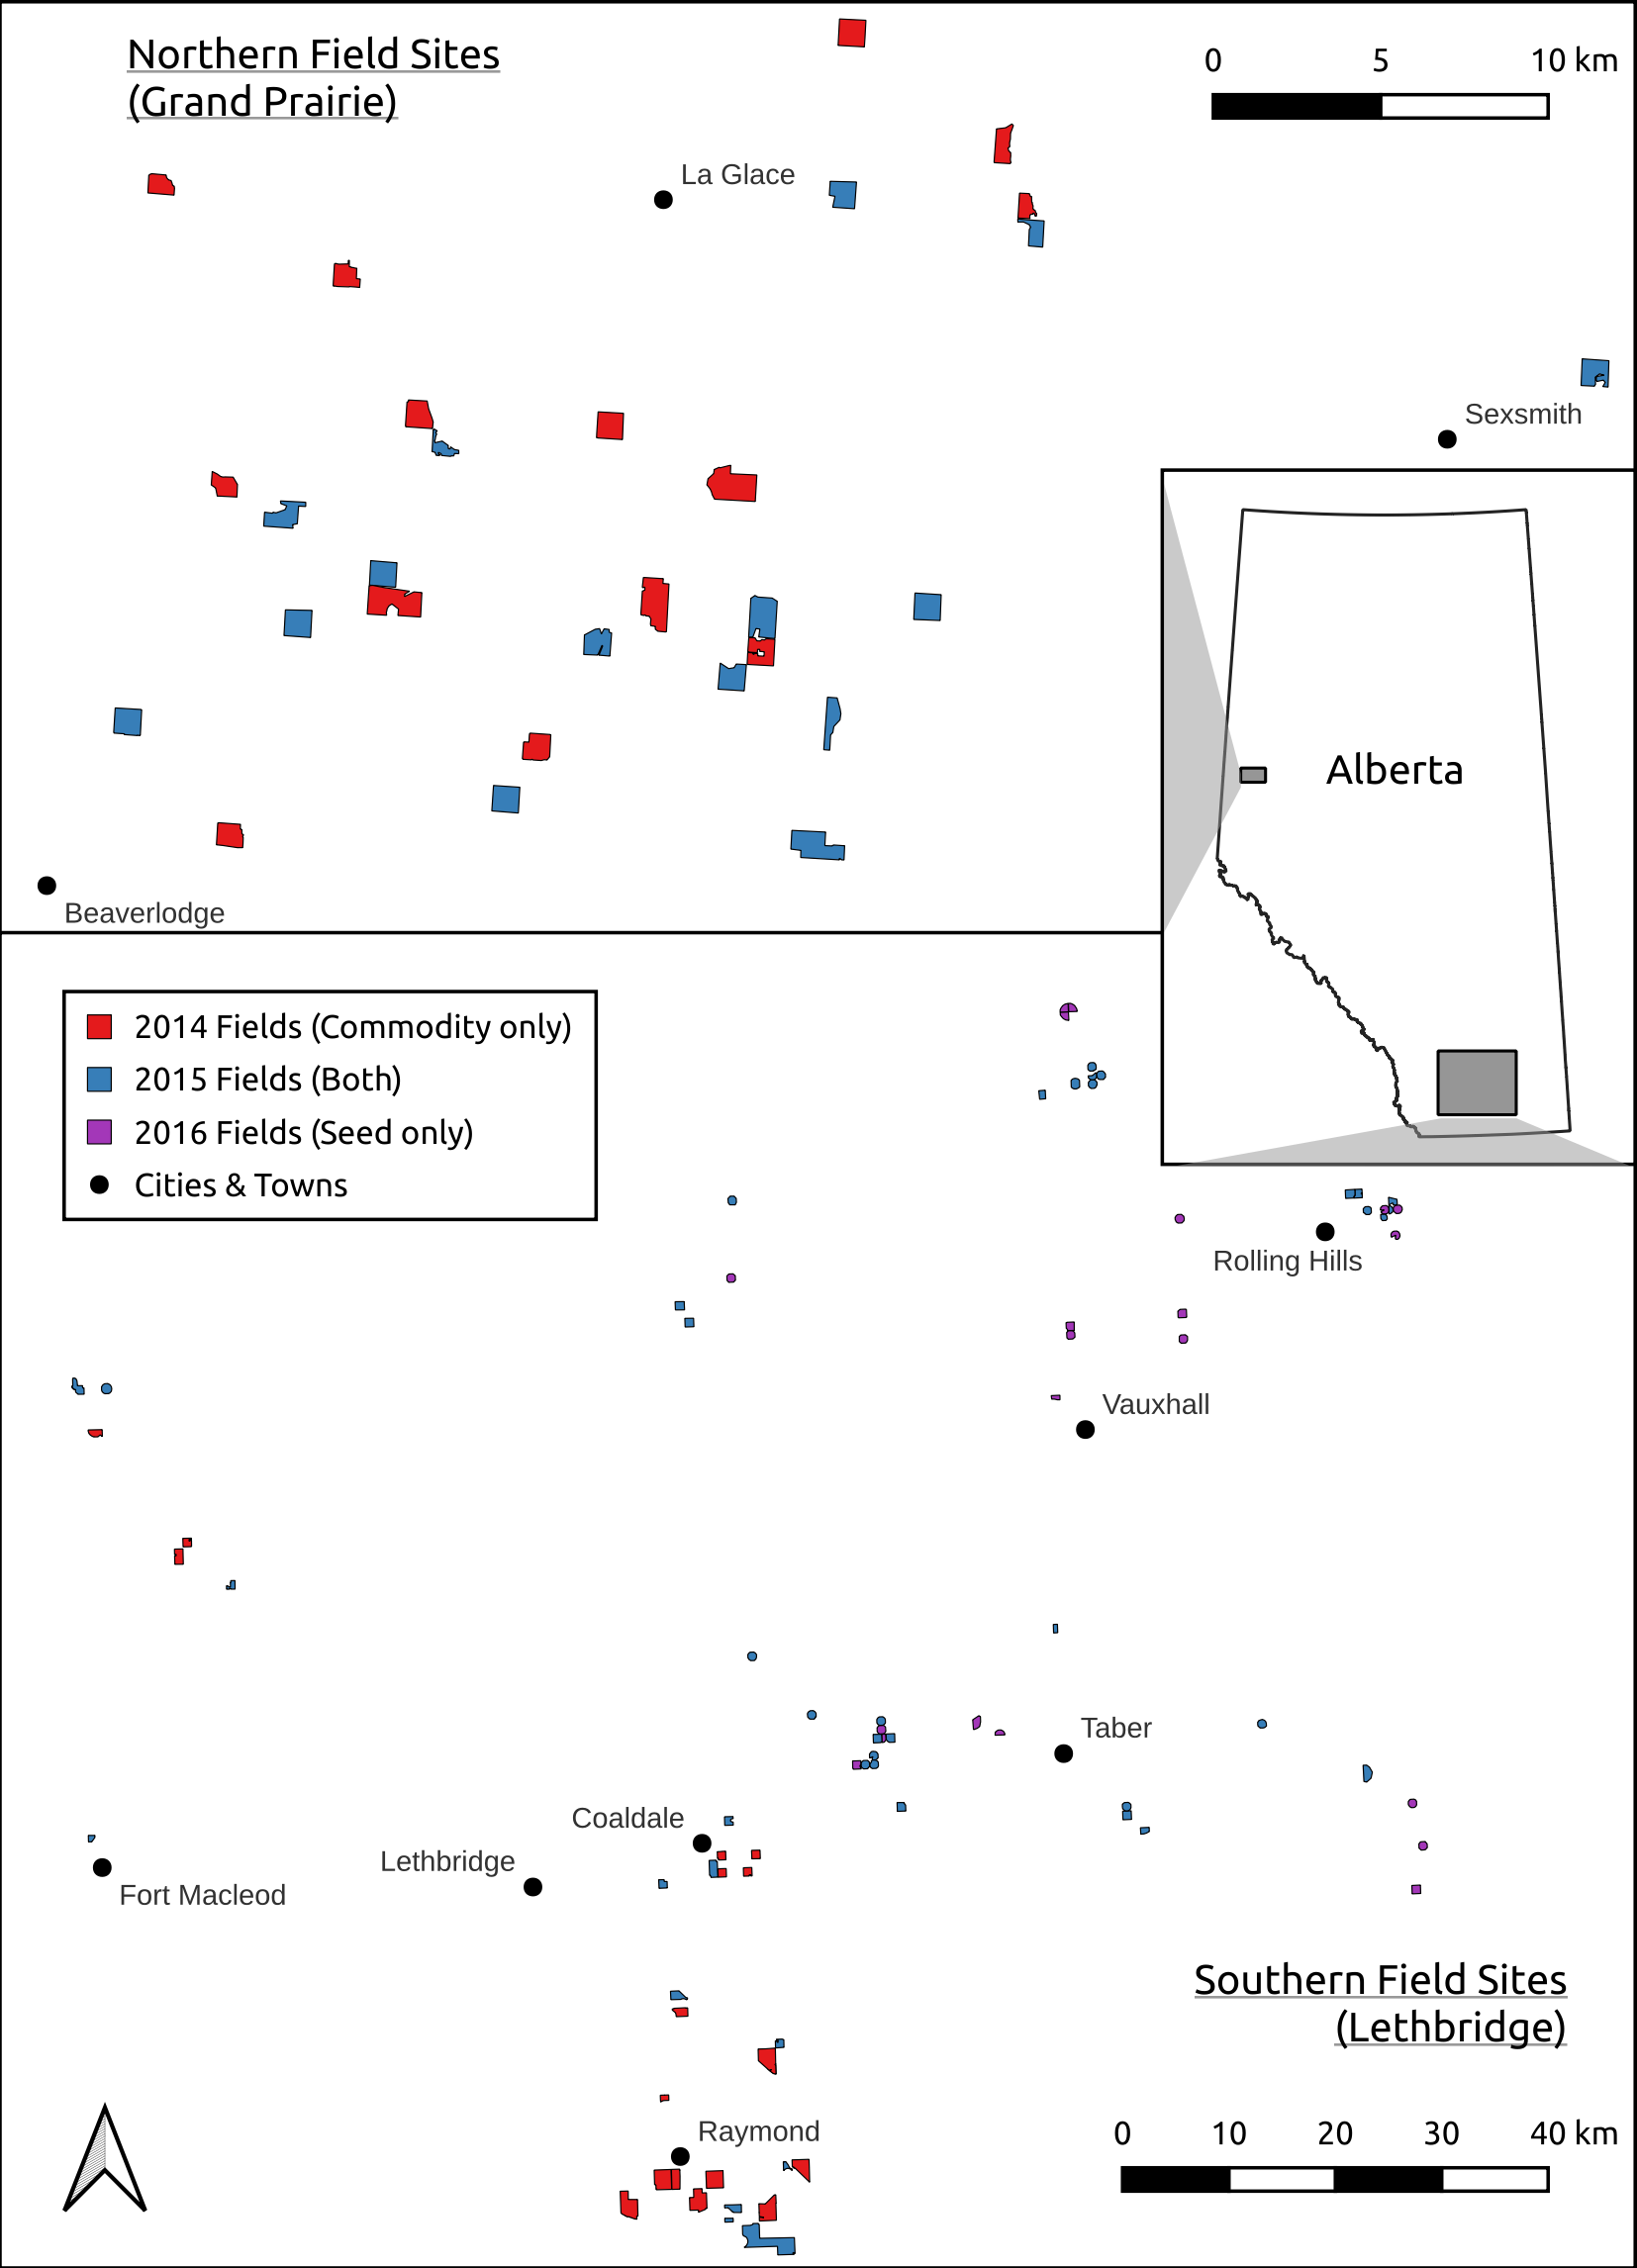
\includegraphics[width=0.9\textwidth,keepaspectratio=true]{FieldLocations.png}
    \caption{Map of sampled fields, showing locations of 29 commodity canola fields (14 during 2014, 15 during 2015), and 35 seed canola fields (15 during 2015, 20 during 2016). Seed canola is grown only in southern Alberta, while commodity canola is grown across both the northern and southern regions.}
\end{figure}


\begin{figure}[h]
    \centering
    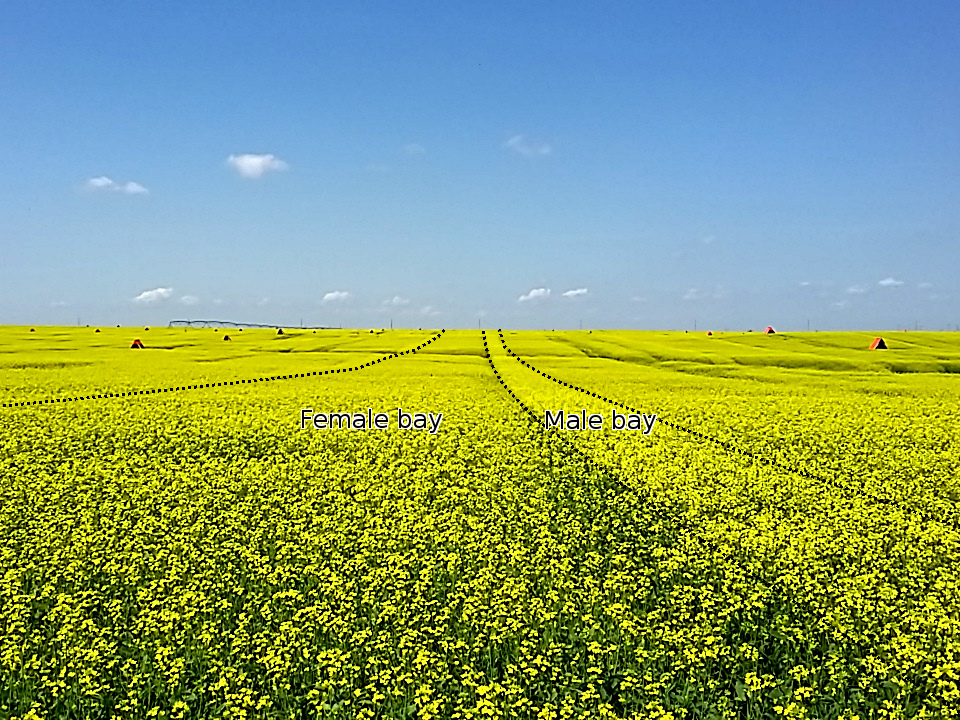
\includegraphics[width=\textwidth,keepaspectratio=true]{seedfieldBays.jpg}
    \caption[Hybrid seed field production field near Rainer, AB]{Hybrid seed field near Rainer, AB, showing the outlines of male and female bays in the foreground, with orange leafcutter bee shelters stationed throughout the field. The linear structure on the horizon is the central-pivot irrigation sprinkler.}
\end{figure}

\begin{figure}[h]
    \centering
    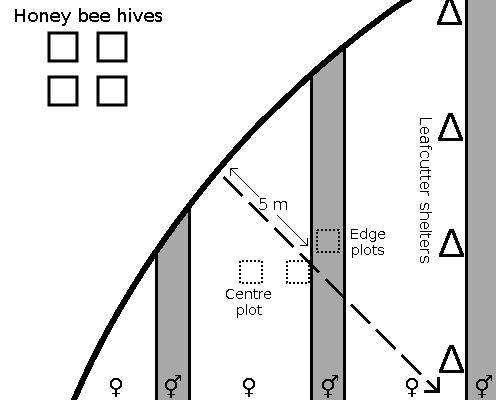
\includegraphics[width=\textwidth,keepaspectratio=true]{seedfieldPlots.png}
    \caption[Plot arrangement for surveys in hybrid seed fields]{Plot arrangement for surveys in hybrid seed fields, showing hypothetical arrangement of leafcutter shelters ($\Delta$), and male-fertile (\Hermaphrodite) and female bays (\Female) at 5m from the edge of the field. Plots were placed along a transect (dashed line) from the field edge nearest to the set of honey bee hives. Plots were placed side-by-side in the male bay and edge of the female bay (``edge" plots), and at the 5m and 400m distances, an additional plot was placed in the centre of the female bay (``centre" plots). Note: this figure shows a small section of a much larger circular field.}
\end{figure}

\begin{table}[h]
\caption{Summary of variables used in structural equation models.}
\centering
\begin{tabular}{l|l|r|r|r|r|r}
\hline
Field Type & Variable & Mean & Median & SD & Min & Max\\
\hline
 & Number of hives & 14.80 & 0.00 & 17.03 & 0.00 & 40.00\\
\cline{2-7}
 & Distance to edge (m) & 137.48 & 20.00 & 195.02 & 1.00 & 500.00\\
\cline{2-7}
 & HB visitation (hr$^{-1}$) & 10.31 & 0.00 & 28.80 & 0.00 & 218.18\\
\cline{2-7}
 & Flower density (m$^2$) & 470.33 & 448.00 & 231.32 & 52.00 & 1684.00\\
\cline{2-7}
 & Pollen per stigma & 293.33 & 155.00 & 385.04 & 0.00 & 3891.00\\
\cline{2-7}
 & Plant density (m$^2$) & 3.77 & 3.77 & 0.48 & 1.79 & 5.02\\
\cline{2-7}
 & Plant vegetative mass (g) & 18.15 & 14.32 & 14.07 & 0.77 & 107.66\\
\cline{2-7}
 & Plant seed mass (g) & 6.87 & 5.46 & 5.97 & 0.01 & 47.90\\
\cline{2-7}
 & Harvest index (g/g) & 0.38 & 0.37 & 0.16 & 0.00 & 1.89\\
\cline{2-7}
 & Flowers per plant & 196.09 & 156.50 & 150.96 & 13.00 & 1094.00\\
\cline{2-7}
 & Pods per plant & 143.15 & 112.00 & 114.64 & 5.00 & 892.00\\
\cline{2-7}
 & Seeds per pod & 22.96 & 23.60 & 4.97 & 4.60 & 35.40\\
\cline{2-7}
\multirow{-13}{*}{\raggedright\arraybackslash Commodity} & Seed size (mg) & 2.74 & 2.73 & 0.80 & 0.39 & 5.35\\
\cline{1-7}
 & Distance to edge (m) & 162.70 & 100.00 & 146.18 & 3.00 & 400.00\\
\cline{2-7}
 & Distance to LCB shelter (m) & 33.51 & 31.00 & 24.63 & 2.00 & 190.00\\
\cline{2-7}
 & HB visitation (hr$^{-1}$) & 112.79 & 24.00 & 187.30 & 0.00 & 1290.00\\
\cline{2-7}
 & LCB visitation (hr$^{-1}$) & 76.15 & 12.00 & 144.88 & 0.00 & 1272.00\\
\cline{2-7}
 & Bay Edge/Centre & 0.13 & 0.00 & 0.34 & 0.00 & 1.00\\
\cline{2-7}
 & Flower density (m$^2$) & 495.02 & 432.00 & 303.35 & 24.00 & 2686.40\\
\cline{2-7}
 & Pollen per stigma & 21.76 & 7.00 & 42.53 & 0.00 & 578.00\\
\cline{2-7}
 & Plant density (m$^2$) & 3.58 & 3.64 & 0.46 & 2.40 & 4.49\\
\cline{2-7}
 & Plant vegetative mass (g) & 30.32 & 25.19 & 21.16 & 1.18 & 144.32\\
\cline{2-7}
 & Plant seed mass (g) & 9.50 & 7.54 & 7.90 & 0.02 & 60.77\\
\cline{2-7}
 & Harvest index (g/g) & 0.32 & 0.33 & 0.15 & 0.00 & 1.21\\
\cline{2-7}
 & Flowers per plant & 461.32 & 362.50 & 326.59 & 26.00 & 2712.00\\
\cline{2-7}
 & Pods per plant & 299.41 & 244.50 & 207.68 & 10.00 & 1410.00\\
\cline{2-7}
 & Seeds per pod & 16.40 & 16.60 & 5.52 & 1.80 & 30.60\\
\cline{2-7}
\multirow{-15}{*}{\raggedright\arraybackslash Seed} & Seed size (mg) & 3.43 & 3.42 & 0.88 & 1.04 & 5.59\\
\hline
\end{tabular}
\end{table}

\clearpage

\section*{Appendix B: Additional information on insect visitors}

In 2015, we recorded whether honey bees were top-working or side-working flowers (see also \citealp{free1973, free1983, mohr1988}).
Top-working bees landed on the top of the flower and inserted their proboscis down between the petals to access the nectaries of the flower, while side-working bees landed on the side of the flower and stole nectar by inserted their proboscis between the petals, avoiding contact with the stigma or anthers. 
Additionally, we recorded whether honey bees were pollen or nectar foragers (pollen foragers had a visible pollen load on their corbicula, while nectar foragers had none).

Pollen- and nectar-foraging honey bees had different patterns of side-working, both on commodity canola, and the male and female lines of seed canola.
Side-working was common in nectar foragers, but was more common in commodity canola (64\%) than in the male (36\%) or female bays (2.8\%) of seed canola, indicating that a large proportion of honey bees foraging on canola flowers may never come in contact with the stigmas.
Pollen foragers were almost uniformly top-foragers in both commodity and seed fields (Table \ref{tab:sideWorking}), and pollen foragers were much less common in the female bays (1.4\%) than in the male bays (15\%), or in commodity fields (18\%).
Therefore, foraging honey bees in seed canola fields tend to treat male-fertile flowers similar to commodity canola flowers, but seem to top-work flowers more in commodity canola than seed fields.
Leafcutter bee foraging behaviours were not recorded, but seemed to almost exclusively top-work flowers in seed canola fields.

\begin{table}[h]
  \caption{Number of flower visitors recorded over a total of 44.8 hours of observation in commodity fields (2014 and 2015), and 46.9 hours of observation in the seed fields (2015 and 2016). ``Fly" refers to larger calyptrate muscoid flies (families Muscidae, Anthomyiidae, Caliphoridae), while ``Hover fly" refers to Syrphid flies. ``Other bee" included Halictid and Andrenid bees, while ``Bumble bee" was \textit{Bombus} spp. ``Butterfly" refers to all visiting Lepidopterans, mostly Pierids.}
  \centering
    \begin{tabular}{r|r|l|r|l}
     & \multicolumn{2}{c|}{Commodity fields} & \multicolumn{2}{c}{Seed fields} \\ \cline{2-5}
    Taxon & Visits & \% & Visits & \% \\ \hline
    Honey bee & 470 & 53.5 & 4850 & 77.1 \\
    Fly & 222 & 25.3 & 74 & 0.878 \\
    Hover fly & 94 & 10.7 & 151 & 1.79 \\
    Other bee & 47 & 5.35 & 30 & 0.356 \\
    Bumble bee & 25 & 2.85 & 0 & 0 \\
    Butterfly & 16 & 1.82 & 0 & 0 \\
    Leafcutter bee & 4 & 0.456 & 1675 & 19.9 \\
    % \hline
    % Total & 828 & - & 6780 & - \\
    \end{tabular}
\end{table}

\begin{table}[h]
\caption[Foraging behaviours of honey bees on commodity and seed canola flowers]{Foraging behaviours of honey bees on commodity and seed canola flowers, recorded during 2015. ``Top" (top-working) indicates that the bee inserted their proboscis down between the petals from the top of the flower, while ``side" (side-working) indicates that the bee fed from the side of the flower and did not contact the anthers or stigma. Pollen foragers had pollen visible on their corbicula, while nectar foragers had none.}
\begin{tabular}{r|r|l|r|l|r|l}
               & \multicolumn{2}{c|}{Commodity fields} & \multicolumn{2}{c|}{Seed fields (female bay)} & \multicolumn{2}{c}{Seed fields (male bay)} \\ \cline{2-7}
               & Top & Side & Top & Side & Top & Side           \\ \hline
Pollen forager & 44 & 2 & 12 & 0 & 115 & 0 \\
Nectar forager & 75 & 138 & 832 & 24 & 428 & 242 \\
% Total & 119 & 140 & 844 & 24 & 543 & 242
\end{tabular}
\end{table}

\clearpage

\section*{Appendix C: Additional information on models}

\subsection*{Commodity canola models}

Formulas for commodity canola model using \texttt{lmer}-style R formulas. Terms on right side of $\sim$ indicate fixed effects, while terms in brackets indicate random effects (heirarchical intercepts). \textit{distribution} indicates the type of probability distribution function used to model each variable.

\begin{align*}
    \text{Plant Density} \sim & \text{HB Distance} + (1|\text{Field}), \text{distribution = log-normal} \\
    \text{Plant Size} \sim & \text{Plant Density} + \text{HB Distance} + (1|\text{Field}),\text{distribution = log-normal} \\
    \text{Flower Density} \sim & \text{Plant Size} + \text{HB Distance} + \text{Plant Density} + (1|\text{Field}),\\
    &   \text{distribution = square root-normal} \\
    \text{HB Visits} \sim & \text{offset}(log(\text{Time})) + \text{HB Distance} + \text{Hive Stocking} + \\ 
    &   \text{Flower Density} + (1|\text{Field}), \text{family = negative binomial}\\
    \text{Pollen per Stigma} \sim & \text{HB Visits} + \text{HB Distance} + (1|\text{Field}), \text{distribution = negative binomial} \\
    \text{Flowers per Plant} \sim & \text{Plant Size} + \text{\% Pod Set} + (1|\text{Field}), \phi \sim \text{Plant Size}, \\
    &     \text{distribution = negative binomial} \\
    \text{\% Pod Set} \sim & \text{HB Visits} + \text{Pollen} + \text{Plant Size} + (1|\text{Field}), \text{distribution = beta-binomial} \\
    \text{Seeds per Pod} \sim & \text{HB Visits} + \text{Pollen} + \text{Plant Size} + \text{\% Pod Set} + \text{Flowers per Plant} + (1|\text{Field}),\\ 
    &   \text{distribution = exponential-normal} \\
    \text{Weight per Seed} \sim & \text{HB Visits} + \text{Pollen} + \text{Seeds per Pod} + \text{Plant Size} + \text{Plant Density} +\\
    &   \text{HB Distance} + \text{\% Pod Set} + \text{Flowers per Plant} + \text{Flower Density} + (1|\text{Field}),\\
    &   \text{distribution = exponential-normal} \\
\end{align*}

\begingroup\fontsize{9}{11}\selectfont

% \begin{longtable}{l|l|r|r|r|r|r|l|r|r} %First manuscript
% \caption{Summary of parameters for commodity canola models} \\
% \hline
% Model & Parameter & Mean & SD & Median & Min & Max & P-value & N$_{eff}$ & $\hat{R}$\\
% \hline
% \endfirsthead
% \multicolumn{10}{@{}l}{\textit{(continued)}}\\
% \hline
% Model & Parameter & Mean & SD & Median & Min & Max & P-value & N$_{eff}$ & $\hat{R}$\\
% \hline
% \endhead
%  & Intercept & 3.76 & 0.05 & 3.77 & 3.66 & 3.87 & $<$0.0001 & 855 & 1.005\\
% \cline{2-10}
%  & HB distance & 0.02 & 0.01 & 0.02 & 0.00 & 0.04 & 0.0868 & 10154 & 1.000\\
% \cline{2-10}
%  & Sigma & 0.31 & 0.02 & 0.31 & 0.28 & 0.34 & - & 5039 & 0.999\\
% \cline{2-10}
% \multirow{-4}{*}{\raggedright\arraybackslash Plant density} & Sigma (field) & 0.37 & 0.04 & 0.37 & 0.30 & 0.46 & - & 3774 & 1.000\\
% \cline{1-10}
%  & Intercept & 5.24 & 0.24 & 5.24 & 4.77 & 5.72 & $<$0.0001 & 2108 & 1.001\\
% \cline{2-10}
%  & Plant density & -0.70 & 0.06 & -0.70 & -0.82 & -0.57 & $<$0.0001 & 2097 & 1.001\\
% \cline{2-10}
%  & HB distance & 0.03 & 0.01 & 0.03 & 0.01 & 0.06 & 0.0095 & 9212 & 1.000\\
% \cline{2-10}
%  & Sigma (field) & 0.22 & 0.04 & 0.22 & 0.15 & 0.29 & - & 1456 & 1.000\\
% \cline{2-10}
% \multirow{-5}{*}{\raggedright\arraybackslash Plant size} & Sigma & 0.64 & 0.02 & 0.64 & 0.61 & 0.68 & - & 7845 & 0.999\\
% \cline{1-10}
%  & Intercept & 5.74 & 4.70 & 5.70 & -3.62 & 15.01 & 0.222 & 1822 & 1.001\\
% \cline{2-10}
%  & Plant size & -1.66 & 0.98 & -1.66 & -3.60 & 0.25 & 0.0926 & 1632 & 1.001\\
% \cline{2-10}
%  & HB distance & 0.75 & 0.11 & 0.75 & 0.53 & 0.96 & $<$0.0001 & 6878 & 1.000\\
% \cline{2-10}
%  & Plant density & -0.41 & 0.74 & -0.42 & -1.86 & 1.06 & 0.5792 & 2243 & 1.001\\
% \cline{2-10}
%  & Sigma & 3.52 & 0.17 & 3.51 & 3.19 & 3.87 & - & 4976 & 0.999\\
% \cline{2-10}
% \multirow{-6}{*}{\raggedright\arraybackslash Flower density} & Sigma (field) & 3.55 & 0.39 & 3.53 & 2.88 & 4.40 & - & 4133 & 1.000\\
% \cline{1-10}
%  & Intercept & -1.98 & 0.45 & -1.96 & -2.89 & -1.17 & $<$0.0001 & 936 & 1.006\\
% \cline{2-10}
%  & HB distance & -0.31 & 0.10 & -0.31 & -0.50 & -0.13 & 0.0011 & 3526 & 1.001\\
% \cline{2-10}
%  & Number of hives & 0.72 & 0.15 & 0.72 & 0.43 & 1.04 & $<$0.0001 & 1534 & 1.003\\
% \cline{2-10}
%  & Flower density & 0.03 & 0.04 & 0.03 & -0.06 & 0.12 & 0.541 & 2397 & 1.000\\
% \cline{2-10}
%  & Sigma (field) & 1.44 & 0.34 & 1.43 & 0.80 & 2.14 & - & 494 & 1.014\\
% \cline{2-10}
% \multirow{-6}{*}{\raggedright\arraybackslash HB visits} & Phi & 0.35 & 0.08 & 0.34 & 0.22 & 0.53 & - & 1630 & 1.003\\
% \cline{1-10}
%  & Intercept & 2.56 & 0.04 & 2.56 & 2.50 & 2.63 & $<$0.0001 & 594 & 1.006\\
% \cline{2-10}
%  & Plant size & 0.94 & 0.01 & 0.94 & 0.92 & 0.96 & $<$0.0001 & 1709 & 1.002\\
% \cline{2-10}
%  & Pods per plant & -0.16 & 0.01 & -0.16 & -0.19 & -0.14 & $<$0.0001 & 2108 & 1.003\\
% \cline{2-10}
%  & Phi (field) & 0.16 & 0.02 & 0.16 & 0.13 & 0.19 & - & 3461 & 1.000\\
% \cline{2-10}
%  & Intercept (Phi) & 2.17 & 0.32 & 2.17 & 1.56 & 2.81 & - & 1517 & 1.001\\
% \cline{2-10}
%  & Plant size (Phi) & 0.66 & 0.11 & 0.66 & 0.44 & 0.87 & - & 1587 & 1.002\\
% \cline{2-10}
% \multirow{-7}{*}{\raggedright\arraybackslash Flowers per plant} & SigmaPhi (field) & 0.66 & 0.12 & 0.65 & 0.45 & 0.90 & - & 844 & 1.005\\
% \cline{1-10}
%  & Intercept & 0.66 & 0.08 & 0.66 & 0.50 & 0.82 & $<$0.0001 & 1946 & 0.999\\
% \cline{2-10}
%  & HB visits & 0.00 & 0.03 & 0.00 & -0.05 & 0.05 & 0.96 & 3292 & 1.000\\
% \cline{2-10}
%  & Plant size & 0.13 & 0.03 & 0.13 & 0.08 & 0.18 & $<$0.0001 & 3345 & 1.000\\
% \cline{2-10}
%  & Pollen count & 0.16 & 0.11 & 0.15 & -0.05 & 0.38 & 0.1515 & 638 & 1.002\\
% \cline{2-10}
%  & Sigma (field) & 0.29 & 0.03 & 0.29 & 0.23 & 0.37 & - & 2675 & 1.000\\
% \cline{2-10}
% \multirow{-6}{*}{\raggedright\arraybackslash Pods per plant} & Phi & 3.35 & 0.07 & 3.35 & 3.21 & 3.48 & - & 3828 & 1.003\\
% \cline{1-10}
%  & Intercept & 25.07 & 1.77 & 25.07 & 21.64 & 28.54 & $<$0.0001 & 2277 & 1.000\\
% \cline{2-10}
%  & HB visits & 0.17 & 0.21 & 0.17 & -0.24 & 0.60 & 0.4284 & 4417 & 1.000\\
% \cline{2-10}
%  & Pollen count & -0.97 & 0.84 & -0.98 & -2.60 & 0.68 & 0.2447 & 707 & 1.003\\
% \cline{2-10}
%  & Plant size & 4.31 & 0.65 & 4.31 & 3.03 & 5.58 & $<$0.0001 & 2229 & 1.000\\
% \cline{2-10}
%  & Pods per plant & 0.56 & 0.29 & 0.56 & 0.00 & 1.12 & 0.0529 & 4888 & 0.999\\
% \cline{2-10}
%  & Flowers per plant & -2.80 & 0.65 & -2.79 & -4.08 & -1.55 & $<$0.0001 & 2105 & 1.000\\
% \cline{2-10}
%  & Sigma & 4.06 & 0.12 & 4.06 & 3.83 & 4.29 & - & 6604 & 1.000\\
% \cline{2-10}
%  & Sigma (field) & 1.98 & 0.26 & 1.96 & 1.51 & 2.53 & - & 2526 & 0.999\\
% \cline{2-10}
% \multirow{-9}{*}{\raggedright\arraybackslash Seeds per pod} & Lambda & 2.00 & 1.03 & 1.74 & 0.84 & 4.64 & - & 3265 & 1.000\\
% \cline{1-10}
%  & Intercept & 0.64 & 0.54 & 0.64 & -0.40 & 1.72 & 0.2367 & 1402 & 1.000\\
% \cline{2-10}
%  & HB visits & 0.02 & 0.04 & 0.02 & -0.05 & 0.09 & 0.6113 & 2748 & 1.000\\
% \cline{2-10}
%  & Pollen count & -0.15 & 0.17 & -0.15 & -0.48 & 0.20 & 0.3744 & 358 & 1.008\\
% \cline{2-10}
%  & Seeds per pod & 0.00 & 0.01 & 0.00 & -0.01 & 0.02 & 0.4508 & 3348 & 1.000\\
% \cline{2-10}
%  & Plant size & -0.03 & 0.12 & -0.03 & -0.26 & 0.20 & 0.7955 & 1633 & 1.000\\
% \cline{2-10}
%  & Plant density & 0.30 & 0.08 & 0.30 & 0.14 & 0.45 & 0.0001 & 1704 & 1.001\\
% \cline{2-10}
%  & HB distance & 0.02 & 0.01 & 0.02 & -0.01 & 0.05 & 0.1686 & 1404 & 1.003\\
% \cline{2-10}
%  & Pods per plant & 0.11 & 0.04 & 0.11 & 0.02 & 0.19 & 0.0159 & 3037 & 1.000\\
% \cline{2-10}
%  & Flowers per plant & 0.11 & 0.12 & 0.11 & -0.13 & 0.34 & 0.363 & 1526 & 1.000\\
% \cline{2-10}
%  & Flower density & -0.03 & 0.01 & -0.03 & -0.04 & -0.02 & $<$0.0001 & 2213 & 1.003\\
% \cline{2-10}
%  & Sigma & 0.52 & 0.03 & 0.52 & 0.46 & 0.59 & - & 2100 & 1.000\\
% \cline{2-10}
%  & Sigma (field) & 0.47 & 0.05 & 0.47 & 0.37 & 0.58 & - & 2828 & 0.999\\
% \cline{2-10}
% \multirow{-13}{*}{\raggedright\arraybackslash Seed size} & Lambda & 2.71 & 0.48 & 2.63 & 2.08 & 3.86 & - & 1792 & 1.001\\
% \hline
% \end{longtable}
% \endgroup{}

\clearpage

\begingroup\fontsize{9}{11}\selectfont
\begin{longtable}{l|l|r|r|l|l|l}
\caption{Summary of parameters for commodity canola models. p-values indicate whether means differed from zero (variance terms were excluded). Means are also shown for 2014 and 2015 models, with * indicating whether parameters differed between years (i.e. posterior 95\% quantiles did not overlap).} \\
\hline
Model & Parameter & Mean & SD & p-value & Mean$_{2014}$ & Mean$_{2015}$\\
\hline
\endfirsthead
\multicolumn{7}{@{}l}{\textit{(continued)}}\\
\hline
Model & Parameter & Mean & SD & p-value & Mean$_{2014}$ & Mean$_{2015}$\\
\hline
\endhead
 & HB distance & 0.016 & 0.010 & 0.0868 & 0.02 & 0.012\\
\cline{2-7}
 & Sigma & 0.309 & 0.016 & - & 0.307 & 0.318\\
\cline{2-7}
\multirow{-3}{*}{\raggedright\arraybackslash Plant density} & Sigma (field) & 0.371 & 0.040 & - & 0.387 & 0.365\\
\cline{1-7}
 & Plant density & -0.695 & 0.063 & $<$0.0001 & -0.826 & -0.492\\
\cline{2-7}
 & HB distance & 0.032 & 0.012 & 0.0095 & 0.025 & 0.042\\
\cline{2-7}
 & Sigma (field) & 0.217 & 0.036 & - & 0.189 & 0.196\\
\cline{2-7}
\multirow{-4}{*}{\raggedright\arraybackslash Plant size} & Sigma & 0.640 & 0.018 & - & 0.65 & 0.626\\
\cline{1-7}
 & Plant size & -1.658 & 0.985 & 0.0926 & -0.602 & -2.193\\
\cline{2-7}
 & HB distance & 0.750 & 0.111 & $<$0.0001 & 0.885 & 0.518\\
\cline{2-7}
 & Plant density & -0.409 & 0.737 & 0.5792 & -0.573 & 0.279\\
\cline{2-7}
 & Sigma & 3.520 & 0.171 & - & 3.965* & 2.663*\\
\cline{2-7}
\multirow{-5}{*}{\raggedright\arraybackslash Flower density} & Sigma (field) & 3.554 & 0.389 & - & 3.779 & 2.834\\
\cline{1-7}
 & HB distance & -0.313 & 0.096 & 0.0011 & -0.442 & -0.262\\
\cline{2-7}
 & Number of hives & 0.720 & 0.153 & $<$0.0001 & 0.848 & 0.654\\
\cline{2-7}
 & Flower density & 0.028 & 0.045 & 0.541 & 0.137 & -0.117\\
\cline{2-7}
 & Sigma (field) & 1.441 & 0.340 & - & 1.019 & 1.383\\
\cline{2-7}
\multirow{-5}{*}{\raggedright\arraybackslash HB visits} & Phi & 0.350 & 0.080 & - & 0.29 & 0.396\\
\cline{1-7}
 & Plant size & 0.937 & 0.010 & $<$0.0001 & 0.935 & 0.946\\
\cline{2-7}
 & Pods per plant & -0.162 & 0.013 & $<$0.0001 & -0.136* & -0.242*\\
\cline{2-7}
 & Phi (field) & 0.160 & 0.016 & - & 0.141 & 0.165\\
\cline{2-7}
 & Plant size (Phi) & 0.659 & 0.110 & - & 0.884* & 0.196*\\
\cline{2-7}
\multirow{-5}{*}{\raggedright\arraybackslash Flowers per plant} & SigmaPhi (field) & 0.660 & 0.116 & - & 0.61 & 0.897\\
\cline{1-7}
 & HB visits & 0.001 & 0.026 & 0.96 & 0.003 & 0.033\\
\cline{2-7}
 & Plant size & 0.133 & 0.026 & $<$0.0001 & 0.108 & 0.167\\
\cline{2-7}
 & Pollen count & 0.158 & 0.110 & 0.1515 & 0.244 & 0.045\\
\cline{2-7}
 & Sigma (field) & 0.294 & 0.034 & - & 0.351 & 0.231\\
\cline{2-7}
\multirow{-5}{*}{\raggedright\arraybackslash Pods per plant} & Phi & 3.346 & 0.067 & - & 3.036* & 3.975*\\
\cline{1-7}
 & HB visits & 0.170 & 0.214 & 0.4284 & 0.262 & 0.342\\
\cline{2-7}
 & Pollen count & -0.974 & 0.837 & 0.2447 & 0.219 & -2.117\\
\cline{2-7}
 & Plant size & 4.310 & 0.650 & $<$0.0001 & 3.855 & 2.899\\
\cline{2-7}
 & Pods per plant & 0.557 & 0.288 & 0.0529 & 0.722 & 0.623\\
\cline{2-7}
 & Flowers per plant & -2.799 & 0.648 & $<$0.0001 & -2.221 & -1.576\\
\cline{2-7}
 & Sigma & 4.057 & 0.117 & - & 4.243 & 3.744\\
\cline{2-7}
 & Sigma (field) & 1.976 & 0.261 & - & 1.591 & 1.517\\
\cline{2-7}
\multirow{-8}{*}{\raggedright\arraybackslash Seeds per pod} & Lambda & 2.001 & 1.029 & - & 1.714 & 1.855\\
\cline{1-7}
 & HB visits & 0.019 & 0.037 & 0.6113 & -0.033 & 0.027\\
\cline{2-7}
 & Pollen count & -0.152 & 0.171 & 0.3744 & -0.341 & 0.147\\
\cline{2-7}
 & Seeds per pod & 0.004 & 0.006 & 0.4508 & -0.001 & 0.014\\
\cline{2-7}
 & Plant size & -0.031 & 0.118 & 0.7955 & 0.143 & -0.332\\
\cline{2-7}
 & Plant density & 0.298 & 0.078 & 0.0001 & 0.289 & 0.353\\
\cline{2-7}
 & HB distance & 0.021 & 0.015 & 0.1686 & -0.013 & 0.076\\
\cline{2-7}
 & Pods per plant & 0.108 & 0.045 & 0.0159 & 0.126 & 0.042\\
\cline{2-7}
 & Flowers per plant & 0.110 & 0.121 & 0.363 & -0.033 & 0.357\\
\cline{2-7}
 & Flower density & -0.030 & 0.007 & $<$0.0001 & -0.022 & -0.04\\
\cline{2-7}
 & Sigma & 0.520 & 0.033 & - & 0.492 & 0.542\\
\cline{2-7}
 & Sigma (field) & 0.468 & 0.052 & - & 0.416 & 0.494\\
\cline{2-7}
\multirow{-12}{*}{\raggedright\arraybackslash Seed size} & Lambda & 2.714 & 0.478 & - & 2.478 & 3.234\\
\hline
\end{longtable}
\endgroup{}

\clearpage

\subsection*{Seed canola models}

Formulas for seed canola model using \texttt{lmer}-style R formulas. Terms on right side of $\sim$ indicate fixed effects, while terms in brackets indicate random effects (heirarchical intercepts). \textit{distribution} indicates the type of probability distribution function used to model each variable.

\begin{align*}
    \text{Plant Density} \sim & \text{HB Distance} + (1|\text{Field}), \text{distribution = log-normal} \\
    \text{Plant Size} \sim & \text{HB Distance} + \text{Plant Density} + (1|\text{Field}) ,\text{distribution = log-t} \\
    \text{Flower Density} \sim & \text{HB Distance} + (1|\text{Field}), \text{distribution = square root-t} \\
    \text{LCB Visits} \sim & \text{offset}(log(\text{Time})) + \text{HB Distance} + \text{LCB Distance} + \text{Bay Centre} + \\
    &   \text{Flower Density} + (1|\text{Field}), \text{family = ZI negative binomial} \\
    \text{HB Visits} \sim & \text{offset}(log(\text{Time})) + \text{HB Distance} + \text{LCB Distance} + \text{Bay Centre} + \\
    &   \text{Flower Density} + (1|\text{Field}), \text{family = ZI negative binomial} \\
    \text{Pollen per Stigma} \sim & \text{HB Visits} + \text{LCB Visits} + \text{Bay Centre} + \text{HB Distance} + \text{LCB Distance} +\\
    &   \text{Flower Density} + (1|\text{Field}) + (1|\text{Plot}), \text{family = negative binomial} \\
    \text{Flowers per Plant} \sim & \text{Plant Size} + \text{Bay Centre} + \text{\% Pod Set} + (1|\text{Field}),\\
    &   \phi \sim \text{Plant Size}, \text{family = negative binomial} \\
    \text{\% Pod Set} \sim & \text{Pollen} + \text{Plant Size} + \text{Bay Centre} + \text{HB Distance} + \text{LCB Distance} + \\
    &   \text{Flower Density} + (1|\text{Field}) + (1|\text{Plot}), \text{family = beta-binomial} \\
    \text{Seeds per Pod} \sim & \text{Pollen} + \text{Plant Size} + \text{Bay Centre} + \text{HB Distance} + \text{Flower Density} +\\
    &   \text{\% Pod Set} + \text{Flowers per plant} + (1|\text{Field}), \text{family = negative binomial} \\
    \text{Weight per Seed} \sim & \text{Pollen} + \text{Seeds per Pod} + \text{Plant Size} + \text{LCB Distance} +\\
    &   \text{Plant Density} + (1|\text{Field}), \text{family = exponential-normal}\\
\end{align*}


% \begingroup\fontsize{9}{11}\selectfont %First manuscript
% \begin{longtable}{l|l|r|r|r|r|r|l|r|r}
% \caption{Summary of parameters for seed canola models} \\
% \hline
% Model & Parameter & Mean & SD & Median & Min & Max & P-value & N$_{eff}$ & $\hat{R}$\\
% \hline
% \endfirsthead
% \multicolumn{10}{@{}l}{\textit{(continued)}}\\
% \hline
% Model & Parameter & Mean & SD & Median & Min & Max & P-value & N$_{eff}$ & $\hat{R}$\\
% \hline
% \endhead
%  & Intercept & 3.60 & 0.06 & 3.60 & 3.47 & 3.73 & $<$0.0001 & 524 & 1.004\\
% \cline{2-10}
%  & HB distance & 0.06 & 0.01 & 0.06 & 0.04 & 0.07 & $<$0.0001 & 5750 & 0.999\\
% \cline{2-10}
%  & Sigma & 0.27 & 0.01 & 0.27 & 0.24 & 0.30 & - & 5199 & 0.999\\
% \cline{2-10}
% \multirow{-4}{*}{\raggedright\arraybackslash Plant density} & Sigma (field) & 0.36 & 0.05 & 0.36 & 0.28 & 0.48 & - & 4182 & 1.000\\
% \cline{1-10}
%  & Intercept & 6.08 & 0.25 & 6.08 & 5.57 & 6.56 & $<$0.0001 & 2480 & 1.000\\
% \cline{2-10}
%  & Plant density & -0.79 & 0.07 & -0.80 & -0.92 & -0.66 & $<$0.0001 & 2470 & 1.000\\
% \cline{2-10}
%  & HB distance & 0.07 & 0.01 & 0.07 & 0.05 & 0.10 & $<$0.0001 & 6446 & 0.999\\
% \cline{2-10}
%  & Sigma & 0.50 & 0.03 & 0.50 & 0.45 & 0.56 & - & 2332 & 1.000\\
% \cline{2-10}
%  & Sigma (field) & 0.15 & 0.04 & 0.15 & 0.08 & 0.23 & - & 1053 & 1.001\\
% \cline{2-10}
% \multirow{-6}{*}{\raggedright\arraybackslash Plant size} & Nu (DF) & 1.91 & 0.32 & 1.87 & 1.37 & 2.65 & $<$0.0001 & 2700 & 1.000\\
% \cline{1-10}
%  & Intercept & 0.48 & 0.56 & 0.46 & -0.58 & 1.64 & 0.3827 & 661 & 1.005\\
% \cline{2-10}
%  & HB distance & 1.11 & 0.12 & 1.11 & 0.87 & 1.36 & $<$0.0001 & 5389 & 1.000\\
% \cline{2-10}
%  & Sigma & 4.06 & 0.24 & 4.05 & 3.59 & 4.56 & - & 2404 & 1.001\\
% \cline{2-10}
%  & Sigma (field) & 3.48 & 0.47 & 3.44 & 2.70 & 4.49 & - & 2640 & 1.001\\
% \cline{2-10}
% \multirow{-5}{*}{\raggedright\arraybackslash Flower density} & Nu (DF) & 1.88 & 0.38 & 1.84 & 1.30 & 2.68 & $<$0.0001 & 1500 & 1.004\\
% \cline{1-10}
%  & Intercept & 3.08 & 0.10 & 3.08 & 2.87 & 3.28 & $<$0.0001 & 2722 & 1.002\\
% \cline{2-10}
%  & Flower density & -0.01 & 0.01 & -0.01 & -0.03 & 0.01 & 0.5267 & 4150 & 1.000\\
% \cline{2-10}
%  & HB distance & -0.02 & 0.05 & -0.03 & -0.12 & 0.07 & 0.6229 & 4410 & 1.000\\
% \cline{2-10}
%  & LCB distance & 0.42 & 0.09 & 0.42 & 0.24 & 0.58 & $<$0.0001 & 5053 & 1.000\\
% \cline{2-10}
%  & Bay centre & 0.45 & 0.21 & 0.45 & 0.07 & 0.88 & 0.0284 & 6486 & 0.999\\
% \cline{2-10}
%  & Phi & 0.72 & 0.09 & 0.72 & 0.55 & 0.92 & - & 4354 & 1.001\\
% \cline{2-10}
%  & Theta (ZI) & 0.32 & 0.03 & 0.32 & 0.26 & 0.38 & - & 3955 & 1.001\\
% \cline{2-10}
% \multirow{-8}{*}{\raggedright\arraybackslash HB visits} & Sigma (field) & 0.41 & 0.11 & 0.41 & 0.22 & 0.64 & - & 600 & 1.001\\
% \cline{1-10}
%  & Intercept & 2.25 & 0.14 & 2.25 & 1.96 & 2.51 & $<$0.0001 & 1734 & 1.002\\
% \cline{2-10}
%  & LCB distance & -0.79 & 0.07 & -0.79 & -0.94 & -0.65 & $<$0.0001 & 4016 & 1.000\\
% \cline{2-10}
%  & HB distance & -0.32 & 0.06 & -0.32 & -0.43 & -0.21 & $<$0.0001 & 5128 & 1.000\\
% \cline{2-10}
%  & Bay centre & -0.34 & 0.23 & -0.34 & -0.77 & 0.16 & 0.1458 & 6667 & 1.000\\
% \cline{2-10}
%  & Flower density & 0.03 & 0.01 & 0.03 & 0.01 & 0.05 & 0.0115 & 4364 & 1.000\\
% \cline{2-10}
%  & Sigma (field) & 0.63 & 0.13 & 0.62 & 0.40 & 0.91 & - & 1072 & 1.004\\
% \cline{2-10}
%  & Phi & 0.70 & 0.11 & 0.69 & 0.50 & 0.93 & - & 3097 & 0.999\\
% \cline{2-10}
% \multirow{-8}{*}{\raggedright\arraybackslash LCB visits} & Theta (ZI) & 0.25 & 0.04 & 0.25 & 0.15 & 0.33 & - & 2383 & 1.000\\
% \cline{1-10}
%  & Intercept & 2.49 & 0.19 & 2.50 & 2.12 & 2.85 & $<$0.0001 & 1141 & 1.002\\
% \cline{2-10}
%  & HB visits & 0.05 & 0.04 & 0.05 & -0.03 & 0.12 & 0.195 & 2317 & 1.000\\
% \cline{2-10}
%  & LCB visits & 0.15 & 0.06 & 0.14 & 0.02 & 0.26 & 0.0155 & 2239 & 1.000\\
% \cline{2-10}
%  & Bay centre & -0.55 & 0.13 & -0.55 & -0.80 & -0.30 & $<$0.0001 & 2540 & 1.000\\
% \cline{2-10}
%  & HB distance & -0.17 & 0.04 & -0.17 & -0.25 & -0.09 & $<$0.0001 & 2265 & 1.003\\
% \cline{2-10}
%  & LCB distance & -0.35 & 0.14 & -0.35 & -0.63 & -0.07 & 0.0164 & 2513 & 1.000\\
% \cline{2-10}
%  & Flower density & -0.03 & 0.02 & -0.03 & -0.06 & 0.01 & 0.1284 & 2058 & 1.001\\
% \cline{2-10}
%  & Sigma (field) & 0.86 & 0.13 & 0.85 & 0.64 & 1.15 & - & 2978 & 1.000\\
% \cline{2-10}
%  & Sigma (plot) & 0.65 & 0.06 & 0.65 & 0.53 & 0.78 & - & 1142 & 1.003\\
% \cline{2-10}
% \multirow{-10}{*}{\raggedright\arraybackslash Pollen count} & Phi & 0.82 & 0.04 & 0.82 & 0.74 & 0.90 & - & 5125 & 0.999\\
% \cline{1-10}
%  & Intercept & 3.05 & 0.04 & 3.05 & 2.96 & 3.14 & $<$0.0001 & 3283 & 0.999\\
% \cline{2-10}
%  & Plant size & 0.93 & 0.01 & 0.93 & 0.90 & 0.95 & $<$0.0001 & 3712 & 0.999\\
% \cline{2-10}
%  & Bay centre & 0.09 & 0.02 & 0.09 & 0.06 & 0.12 & $<$0.0001 & 6790 & 0.999\\
% \cline{2-10}
%  & Pods per plant & -0.14 & 0.01 & -0.14 & -0.17 & -0.12 & $<$0.0001 & 5503 & 0.999\\
% \cline{2-10}
%  & Sigma (field) & 0.08 & 0.01 & 0.08 & 0.06 & 0.11 & - & 2649 & 1.000\\
% \cline{2-10}
%  & Intercept (Phi) & 2.24 & 0.32 & 2.24 & 1.62 & 2.87 & - & 2875 & 1.001\\
% \cline{2-10}
% \multirow{-7}{*}{\raggedright\arraybackslash Flowers per plant} & Plant size (Phi) & 0.38 & 0.10 & 0.39 & 0.19 & 0.57 & - & 2871 & 1.001\\
% \cline{1-10}
%  & Intercept & 0.18 & 0.12 & 0.18 & -0.05 & 0.40 & 0.1211 & 2261 & 1.000\\
% \cline{2-10}
%  & Pollen count & 0.12 & 0.04 & 0.12 & 0.03 & 0.20 & 0.0074 & 915 & 1.004\\
% \cline{2-10}
%  & Plant size & 0.19 & 0.03 & 0.19 & 0.14 & 0.24 & $<$0.0001 & 4570 & 1.000\\
% \cline{2-10}
%  & Bay centre & -0.21 & 0.06 & -0.21 & -0.33 & -0.10 & 0.0003 & 1886 & 1.000\\
% \cline{2-10}
%  & HB distance & -0.12 & 0.02 & -0.12 & -0.15 & -0.08 & $<$0.0001 & 1929 & 1.002\\
% \cline{2-10}
%  & LCB distance & -0.21 & 0.06 & -0.21 & -0.34 & -0.10 & 0.0005 & 2637 & 1.000\\
% \cline{2-10}
%  & Flower density & 0.00 & 0.01 & 0.00 & -0.02 & 0.01 & 0.5456 & 2998 & 1.000\\
% \cline{2-10}
%  & Sigma (plot) & 0.30 & 0.03 & 0.30 & 0.25 & 0.35 & - & 1367 & 1.004\\
% \cline{2-10}
%  & Sigma (field) & 0.37 & 0.06 & 0.36 & 0.27 & 0.49 & - & 2905 & 1.000\\
% \cline{2-10}
%  & Intercept (Phi) & 3.07 & 0.38 & 3.05 & 2.36 & 3.85 & - & 2268 & 1.004\\
% \cline{2-10}
% \multirow{-11}{*}{\raggedright\arraybackslash Pods per plant} & Plant size (Phi) & 0.22 & 0.12 & 0.22 & -0.01 & 0.44 & - & 2538 & 1.003\\
% \cline{1-10}
%  & Intercept & 25.38 & 2.29 & 25.48 & 20.64 & 29.38 & $<$0.0001 & 1651 & 1.001\\
% \cline{2-10}
%  & Pollen count & 1.21 & 0.32 & 1.20 & 0.61 & 1.87 & 0.0001 & 1046 & 1.002\\
% \cline{2-10}
%  & Plant size & 4.76 & 0.78 & 4.76 & 3.24 & 6.23 & $<$0.0001 & 1752 & 1.001\\
% \cline{2-10}
%  & Bay centre & -0.50 & 0.45 & -0.50 & -1.39 & 0.38 & 0.2639 & 5315 & 0.999\\
% \cline{2-10}
%  & HB distance & -0.02 & 0.12 & -0.01 & -0.25 & 0.21 & 0.881 & 3007 & 1.000\\
% \cline{2-10}
%  & Flower density & -0.11 & 0.06 & -0.11 & -0.23 & 0.00 & 0.0451 & 2596 & 1.000\\
% \cline{2-10}
%  & Pods per plant & 1.65 & 0.35 & 1.65 & 0.94 & 2.34 & $<$0.0001 & 2485 & 1.001\\
% \cline{2-10}
%  & Flowers per plant & -4.26 & 0.74 & -4.27 & -5.60 & -2.73 & $<$0.0001 & 1571 & 1.001\\
% \cline{2-10}
%  & Sigma & 4.25 & 0.16 & 4.25 & 3.92 & 4.56 & - & 2951 & 1.000\\
% \cline{2-10}
%  & Sigma (field) & 1.97 & 0.32 & 1.95 & 1.41 & 2.68 & - & 1767 & 1.002\\
% \cline{2-10}
% \multirow{-11}{*}{\raggedright\arraybackslash Seeds per pod} & Lambda & 1.67 & 1.00 & 1.39 & 0.60 & 4.28 & - & 2448 & 0.999\\
% \cline{1-10}
%  & Intercept & 1.17 & 0.50 & 1.18 & 0.21 & 2.16 & 0.0189 & 2004 & 1.001\\
% \cline{2-10}
%  & Pollen count & -0.02 & 0.05 & -0.02 & -0.12 & 0.08 & 0.7002 & 2345 & 1.000\\
% \cline{2-10}
%  & Seeds per pod & -0.01 & 0.01 & -0.01 & -0.03 & 0.00 & 0.0765 & 3719 & 0.999\\
% \cline{2-10}
%  & Plant size & 0.23 & 0.06 & 0.23 & 0.12 & 0.34 & $<$0.0001 & 3607 & 1.000\\
% \cline{2-10}
%  & Plant density & 0.41 & 0.11 & 0.41 & 0.20 & 0.63 & 0.0002 & 1988 & 1.000\\
% \cline{2-10}
%  & LCB distance & 0.07 & 0.07 & 0.07 & -0.06 & 0.22 & 0.3146 & 4466 & 1.000\\
% \cline{2-10}
%  & Sigma & 0.75 & 0.03 & 0.75 & 0.69 & 0.81 & - & 3533 & 1.000\\
% \cline{2-10}
%  & Sigma (field) & 0.36 & 0.06 & 0.35 & 0.25 & 0.49 & - & 2060 & 1.000\\
% \cline{2-10}
% \multirow{-9}{*}{\raggedright\arraybackslash Seed size} & Lambda & 4.44 & 1.22 & 4.23 & 2.70 & 7.42 & - & 2125 & 1.000\\
% \hline
% \end{longtable}
% \endgroup{}

\begingroup\fontsize{9}{11}\selectfont

\begin{longtable}{l|l|r|r|l|l|l}
\caption{Summary of parameters for seed canola models. p-values indicate whether means differed from zero (variance terms were excluded). Means are also shown for 2015 and 2016 models, with * indicating whether parameters differed between years (i.e. posterior 95\% quantiles did not overlap).} \\
\hline
Model & Parameter & Mean & SD & p-value & Mean$_{2015}$ & Mean$_{2016}$\\
\hline
\endfirsthead
\multicolumn{7}{@{}l}{\textit{(continued)}}\\
\hline
Model & Parameter & Mean & SD & p-value & Mean$_{2015}$ & Mean$_{2016}$\\
\hline
\endhead
 & HB distance & 0.055 & 0.010 & $<$0.0001 & 0.075 & 0.041\\
\cline{2-7}
 & Sigma & 0.272 & 0.015 & - & 0.324* & 0.229*\\
\cline{2-7}
\multirow{-3}{*}{\raggedright\arraybackslash Plant density} & Sigma (field) & 0.364 & 0.049 & - & 0.332 & 0.375\\
\cline{1-7}
 & Plant density & -0.794 & 0.069 & $<$0.0001 & -0.65 & -0.912\\
\cline{2-7}
 & HB distance & 0.074 & 0.013 & $<$0.0001 & 0.07 & 0.075\\
\cline{2-7}
 & Sigma & 0.505 & 0.029 & - & 0.561 & 0.491\\
\cline{2-7}
 & Sigma (field) & 0.151 & 0.037 & - & 0.141 & 0.146\\
\cline{2-7}
\multirow{-5}{*}{\raggedright\arraybackslash Plant size} & Nu (DF) & 1.905 & 0.325 & $<$0.0001 & 1.974 & 2.988\\
\cline{1-7}
 & HB distance & 1.109 & 0.124 & $<$0.0001 & 1.481 & 0.982\\
\cline{2-7}
 & Sigma & 4.055 & 0.244 & - & 5.232* & 3.688*\\
\cline{2-7}
 & Sigma (field) & 3.485 & 0.466 & - & 3.483 & 1.976\\
\cline{2-7}
\multirow{-4}{*}{\raggedright\arraybackslash Flower density} & Nu (DF) & 1.875 & 0.376 & $<$0.0001 & 3.045 & 3.999\\
\cline{1-7}
 & Flower density & -0.007 & 0.011 & 0.5267 & -0.018 & 0.033\\
\cline{2-7}
 & HB distance & -0.024 & 0.050 & 0.6229 & -0.128 & 0.012\\
\cline{2-7}
 & LCB distance & 0.415 & 0.085 & $<$0.0001 & 0.421 & 0.403\\
\cline{2-7}
 & Bay centre & 0.452 & 0.206 & 0.0284 & 0.441 & 0.382\\
\cline{2-7}
 & Phi & 0.719 & 0.094 & - & 0.632 & 0.796\\
\cline{2-7}
 & Theta (ZI) & 0.320 & 0.029 & - & 0.291 & 0.328\\
\cline{2-7}
\multirow{-7}{*}{\raggedright\arraybackslash HB visits} & Sigma (field) & 0.413 & 0.108 & - & 0.263 & 0.532\\
\cline{1-7}
 & LCB distance & -0.790 & 0.074 & $<$0.0001 & -0.752 & -0.858\\
\cline{2-7}
 & HB distance & -0.319 & 0.055 & $<$0.0001 & -0.374 & -0.233\\
\cline{2-7}
 & Bay centre & -0.335 & 0.231 & 0.1458 & -0.104 & -0.576\\
\cline{2-7}
 & Flower density & 0.028 & 0.011 & 0.0115 & 0.018 & 0.055\\
\cline{2-7}
 & Sigma (field) & 0.629 & 0.129 & - & 0.617 & 0.602\\
\cline{2-7}
 & Phi & 0.698 & 0.112 & - & 0.717 & 0.643\\
\cline{2-7}
\multirow{-7}{*}{\raggedright\arraybackslash LCB visits} & Theta (ZI) & 0.248 & 0.045 & - & 0.195 & 0.278\\
\cline{1-7}
 & HB visits & 0.050 & 0.039 & 0.195 & 0.038 & 0.079\\
\cline{2-7}
 & LCB visits & 0.146 & 0.060 & 0.0155 & 0.151 & 0.115\\
\cline{2-7}
 & Bay centre & -0.550 & 0.129 & $<$0.0001 & -0.424 & -0.626\\
\cline{2-7}
 & HB distance & -0.169 & 0.039 & $<$0.0001 & -0.166 & -0.171\\
\cline{2-7}
 & LCB distance & -0.348 & 0.145 & 0.0164 & 0.08 & -0.506\\
\cline{2-7}
 & Flower density & -0.026 & 0.017 & 0.1284 & -0.009 & -0.032\\
\cline{2-7}
 & Sigma (field) & 0.862 & 0.130 & - & 0.639 & 0.964\\
\cline{2-7}
 & Sigma (plot) & 0.651 & 0.064 & - & 0.663 & 0.679\\
\cline{2-7}
\multirow{-9}{*}{\raggedright\arraybackslash Pollen count} & Phi & 0.817 & 0.042 & - & 0.958 & 0.724\\
\cline{1-7}
 & Plant size & 0.926 & 0.013 & $<$0.0001 & 0.933 & 0.925\\
\cline{2-7}
 & Bay centre & 0.091 & 0.016 & $<$0.0001 & 0.08 & 0.09\\
\cline{2-7}
 & Pods per plant & -0.141 & 0.012 & $<$0.0001 & -0.215* & -0.118*\\
\cline{2-7}
 & Sigma (field) & 0.082 & 0.014 & - & 0.11 & 0.06\\
\cline{2-7}
\multirow{-5}{*}{\raggedright\arraybackslash Flowers per plant} & Plant size (Phi) & 0.384 & 0.097 & - & 0.606 & 0.14\\
\cline{1-7}
 & Pollen count & 0.119 & 0.044 & 0.0074 & -0.009 & 0.186\\
\cline{2-7}
 & Plant size & 0.190 & 0.027 & $<$0.0001 & 0.216 & 0.147\\
\cline{2-7}
 & Bay centre & -0.212 & 0.059 & 0.0003 & -0.362 & -0.113\\
\cline{2-7}
 & HB distance & -0.115 & 0.019 & $<$0.0001 & -0.118 & -0.131\\
\cline{2-7}
 & LCB distance & -0.214 & 0.062 & 0.0005 & -0.135 & -0.254\\
\cline{2-7}
 & Flower density & -0.005 & 0.008 & 0.5456 & -0.02 & 0.009\\
\cline{2-7}
 & Sigma (plot) & 0.296 & 0.026 & - & 0.259 & 0.32\\
\cline{2-7}
 & Sigma (field) & 0.366 & 0.056 & - & 0.105* & 0.464*\\
\cline{2-7}
\multirow{-9}{*}{\raggedright\arraybackslash Pods per plant} & Plant size (Phi) & 0.222 & 0.115 & - & 0.492 & -0.032\\
\cline{1-7}
 & Pollen count & 1.208 & 0.317 & 0.0001 & 0.369 & 1.48\\
\cline{2-7}
 & Plant size & 4.757 & 0.776 & $<$0.0001 & 4.309 & 3.009\\
\cline{2-7}
 & Bay centre & -0.502 & 0.449 & 0.2639 & -0.621 & -0.655\\
\cline{2-7}
 & HB distance & -0.018 & 0.120 & 0.881 & -0.287 & 0.128\\
\cline{2-7}
 & Flower density & -0.114 & 0.057 & 0.0451 & 0.02 & -0.184\\
\cline{2-7}
 & Pods per plant & 1.647 & 0.352 & $<$0.0001 & 3.201 & 1.305\\
\cline{2-7}
 & Flowers per plant & -4.257 & 0.743 & $<$0.0001 & -3.396 & -2.971\\
\cline{2-7}
 & Sigma & 4.250 & 0.156 & - & 4.14 & 4.252\\
\cline{2-7}
 & Sigma (field) & 1.972 & 0.322 & - & 1.476 & 1.972\\
\cline{2-7}
\multirow{-10}{*}{\raggedright\arraybackslash Seeds per pod} & Lambda & 1.673 & 0.995 & - & 1.5 & 1.453\\
\cline{1-7}
 & Pollen count & -0.020 & 0.051 & 0.7002 & -0.016 & 0.013\\
\cline{2-7}
 & Seeds per pod & -0.013 & 0.007 & 0.0765 & 0.016* & -0.04*\\
\cline{2-7}
 & Plant size & 0.233 & 0.055 & $<$0.0001 & 0.255 & 0.129\\
\cline{2-7}
 & Plant density & 0.413 & 0.110 & 0.0002 & 0.508 & 0.047\\
\cline{2-7}
 & LCB distance & 0.072 & 0.072 & 0.3146 & -0.117 & 0.138\\
\cline{2-7}
 & Sigma & 0.751 & 0.030 & - & 0.768 & 0.686\\
\cline{2-7}
 & Sigma (field) & 0.358 & 0.061 & - & 0.333 & 0.298\\
\cline{2-7}
\multirow{-8}{*}{\raggedright\arraybackslash Seed size} & Lambda & 4.436 & 1.219 & - & 3.491 & 4.191\\
\hline
\end{longtable}
\endgroup{}


\clearpage

\subsection*{Total yield models}

Formulas for total yield models are  using \texttt{lmer}-style R formulas. Predicted yield for each plant was calculated as: pods per plant $\times$ seeds per pod $\times$ weight per seed. Terms on right side of $\sim$ indicate fixed effects, while terms in brackets indicate random intercepts (and slopes). 

\begin{align*}
    \text{Total Yield} \sim & log(\text{Predicted Yield}) + (log(\text{Predicted Yield})|\text{Field}) + \\
    & (log(\text{Predicted Yield})|\text{Plot}), \text{distribution = log-normal} \\
\end{align*}

% \begin{table}[h] %First manuscript
% \centering\begingroup\fontsize{9}{11}\selectfont
% \caption{Summary of parameters for total yield models} 
% \begin{tabular}{l|l|r|r|r|r|r|r|r|r|r}
% \hline
% Field Type & Parameter & Mean & SD & Z & median & Min & Max & p-value & N$_{eff}$ & $\hat{R}$\\
% \hline
%  & Intercept & -0.318 & 0.042 & -7.62 & -0.317 & -0.397 & -0.236 & 0.000 & 982 & 1.000\\
% \cline{2-11}
%  & Predicted Yield & 1.007 & 0.018 & 55.64 & 1.007 & 0.972 & 1.044 & 0.000 & 1044 & 1.000\\
% \cline{2-11}
%  & Sigma (field intercept) & 0.119 & 0.041 & 2.89 & 0.112 & 0.051 & 0.216 & 0.004 & 292 & 1.020\\
% \cline{2-11}
%  & Sigma (field slope) & 0.026 & 0.019 & 1.37 & 0.023 & 0.001 & 0.072 & 0.170 & 295 & 1.013\\
% \cline{2-11}
%  & Sigma (plot intercept) & 0.389 & 0.037 & 10.47 & 0.388 & 0.318 & 0.465 & 0.000 & 506 & 1.005\\
% \cline{2-11}
%  & Sigma (plot slope) & 0.169 & 0.017 & 9.86 & 0.168 & 0.135 & 0.204 & 0.000 & 556 & 1.006\\
% \cline{2-11}
%  & Sigma & 0.253 & 0.008 & 33.30 & 0.253 & 0.239 & 0.268 & 0.000 & 2002 & 1.000\\
% \cline{2-11}
%  & Correlation (Int:Slope field) & -0.400 & 0.448 & -0.89 & -0.525 & -0.944 & 0.626 & 0.372 & 660 & 1.005\\
% \cline{2-11}
% \multirow{-9}{*}{\raggedright\arraybackslash Commodity} & Correlation (Int:Slope plot) & -0.989 & 0.007 & -140.44 & -0.990 & -0.998 & -0.972 & 0.000 & 936 & 1.005\\
% \cline{1-11}
%  & Intercept & -0.210 & 0.072 & -2.90 & -0.210 & -0.348 & -0.066 & 0.004 & 738 & 1.007\\
% \cline{2-11}
%  & Predicted Yield & 0.856 & 0.025 & 34.62 & 0.856 & 0.806 & 0.904 & 0.000 & 672 & 1.008\\
% \cline{2-11}
%  & Sigma (field intercept) & 0.040 & 0.018 & 2.28 & 0.038 & 0.011 & 0.079 & 0.022 & 226 & 1.005\\
% \cline{2-11}
%  & Sigma (field slope) & 0.010 & 0.007 & 1.56 & 0.009 & 0.001 & 0.023 & 0.118 & 217 & 1.005\\
% \cline{2-11}
%  & Sigma (plot intercept) & 0.097 & 0.013 & 7.26 & 0.097 & 0.072 & 0.124 & 0.000 & 470 & 1.005\\
% \cline{2-11}
%  & Sigma (plot slope) & 0.032 & 0.005 & 5.83 & 0.032 & 0.021 & 0.043 & 0.000 & 379 & 1.006\\
% \cline{2-11}
%  & Sigma & 0.289 & 0.012 & 23.59 & 0.289 & 0.266 & 0.314 & 0.000 & 1218 & 1.001\\
% \cline{2-11}
%  & Correlation (Int:Slope field) & -0.470 & 0.436 & -1.08 & -0.616 & -0.946 & 0.603 & 0.281 & 457 & 1.005\\
% \cline{2-11}
% \multirow{-9}{*}{\raggedright\arraybackslash Seed} & Correlation (Int:Slope plot) & -0.902 & 0.038 & -23.81 & -0.909 & -0.954 & -0.808 & 0.000 & 486 & 1.007\\
% \hline
% \end{tabular}
% \label{tab:totalYieldCoefs}
% \endgroup{}
% \end{table}

\begin{table}[h]
\centering\begingroup\fontsize{9}{11}\selectfont
\caption{Summary of parameters for total yield models. p-values indicate whether means differed from zero (variance terms were excluded).}
\begin{tabular}{l|l|r|r|l}
\hline
Field Type & Parameter & Mean & SD & p-value\\
\hline
 & Intercept & -0.318 & 0.042 & $<$0.0001\\
\cline{2-5}
 & Predicted Yield & 1.007 & 0.018 & $<$0.0001\\
\cline{2-5}
 & Sigma (field intercept) & 0.119 & 0.041 & -\\
\cline{2-5}
 & Sigma (field slope) & 0.026 & 0.019 & -\\
\cline{2-5}
 & Sigma (plot intercept) & 0.389 & 0.037 & -\\
\cline{2-5}
 & Sigma (plot slope) & 0.169 & 0.017 & -\\
\cline{2-5}
 & Sigma & 0.253 & 0.008 & -\\
\cline{2-5}
 & Correlation (Int:Slope field) & -0.400 & 0.448 & -\\
\cline{2-5}
\multirow{-9}{*}{\raggedright\arraybackslash Commodity} & Correlation (Int:Slope plot) & -0.989 & 0.007 & -\\
\cline{1-5}
 & Intercept & -0.210 & 0.072 & 0.0037\\
\cline{2-5}
 & Predicted Yield & 0.856 & 0.025 & $<$0.0001\\
\cline{2-5}
 & Sigma (field intercept) & 0.040 & 0.018 & -\\
\cline{2-5}
 & Sigma (field slope) & 0.010 & 0.007 & -\\
\cline{2-5}
 & Sigma (plot intercept) & 0.097 & 0.013 & -\\
\cline{2-5}
 & Sigma (plot slope) & 0.032 & 0.005 & -\\
\cline{2-5}
 & Sigma & 0.289 & 0.012 & -\\
\cline{2-5}
 & Correlation (Int:Slope field) & -0.470 & 0.436 & -\\
\cline{2-5}
\multirow{-9}{*}{\raggedright\arraybackslash Seed} & Correlation (Int:Slope plot) & -0.902 & 0.038 & -\\
\hline
\end{tabular}
\endgroup{}
\end{table}

\bibliographystyle{humanbio}
\begin{thebibliography}{}

\bibitem[\protect\astroncite{Free and Ferguson}{1983}]{free1983}
Free, J.~B. and Ferguson, A.~W. 1983.
\newblock Foraging behaviour of honeybees on oilseed rape.
\newblock {\em Bee World}, 64(1):22--24.

\bibitem[\protect\astroncite{Free and Williams}{1973}]{free1973}
Free, J.~B. and Williams, I.~H. 1973.
\newblock The foraging behaviour of honeybees (\emph{Apis mellifera} {L.}) on
  brussels sprout (\emph{Brassica oleracea} {L.}).
\newblock {\em Journal of Applied Ecology}, 10(2):489--499.

\bibitem[\protect\astroncite{Mohr and Jay}{1988}]{mohr1988}
Mohr, N.~A. and Jay, S.~C. 1988.
\newblock Nectar- and pollen-collecting behaviour of honeybees on canola
  (\emph{Brassica campestris} {L}. and \emph{Brassica napus} {L}.).
\newblock {\em Journal of Apicultural Research}, 27(2):131--136.

\end{thebibliography}


\end{document}

\end{document}